\documentclass[journal]{IEEEtran}

% -------- Packages ---------------------------------------------------
\usepackage[utf8]{inputenc}
\usepackage{amsmath,amssymb,amsthm}
\usepackage{graphicx}
\usepackage{booktabs}
\usepackage{array}
\usepackage{cite}
\usepackage{url}
\usepackage{hyperref}
\usepackage{algorithm}
\usepackage{algpseudocode}
\usepackage{bm}
\usepackage{tikz}
\usetikzlibrary{arrows.meta,positioning,calc,shapes.geometric}

\hypersetup{
  colorlinks=true,
  linkcolor=black,
  citecolor=black,
  urlcolor=blue,
}

% -------- Theorem environments --------------------------------------
\newtheorem{proposition}{Proposition}
\newtheorem{lemma}{Lemma}
\newtheorem{corollary}{Corollary}
\theoremstyle{remark}
\newtheorem{remark}{Remark}

% -------- Math macros -----------------------------------------------
\newcommand{\R}{\mathbb{R}}
\newcommand{\C}{\mathbb{C}}
\newcommand{\Nyq}{f_{\mathrm{N}}}
\DeclareMathOperator{\rFFT}{rFFT}
\DeclareMathOperator{\irFFT}{irFFT}
\DeclareMathOperator{\softmax}{softmax}
\newcommand{\IMF}{\mathrm{IMF}}
\newcommand{\cEMD}{c}

% =====================================================================
\begin{document}

\title{Neural Adaptive Filter Bank: Differentiable Signal
Decomposition via Softmax Partition of Unity}

\author{Aous~A.~Abdo%
\thanks{A.~A.~Abdo is with Analytica Data Science Solutions,
Falls Church, VA 22043, USA (e-mail: aous.abdo@analyticadss.com).}}

\markboth{IEEE Transactions on Signal Processing, Submitted April 2026}%
{Abdo: Neural Adaptive Filter Bank}

\maketitle

% =====================================================================
\begin{abstract}
We present Neural Adaptive Filter Bank (NAFB), a differentiable
signal-adaptive filter bank whose architecture guarantees three
properties by construction, without relying on any loss to enforce
them: exact reconstruction of the input signal, a Parseval--Cauchy--Schwarz
upper bound on the total energy of the components, and non-negative
bandpass filter responses. Pairwise orthogonality is a corollary that
becomes exact as the softmax temperature tends to zero. A small 1D
convolutional analyzer reads the magnitude and phase of the input
spectrum and predicts $K$ log-responses; a softmax over the $K$
dimension produces a partition of unity in the frequency domain, and
the inverse FFT of each filtered spectrum yields an intrinsic mode
function. The guarantees hold at initialisation, during training, and
on unseen inputs. We also report a negative result that motivates the
architectural approach: a generic iterative sifting network trained
with seven soft physics losses kept finding a new degenerate minimum
whenever an additional loss was added, because soft constraints do
not shrink the feasible set of a non-convex optimisation.
Architectural constraints do. On a multi-seed three-class classification benchmark with a
head-matched VMD$+$MLP baseline, end-to-end NAFB beats the
baseline at SNR $3$\,dB ($94.97 \pm 1.09$ vs.\ $92.67 \pm 0.78$\,\%,
$+2.3$\,pp over the baseline)
and loses by $3.3$ and $3.6$ pp at $10$ and $20$\,dB in the
near-ceiling regime where every decomposition-based method sits above
$92$\,\%. Generic learnable filter banks (mel-scale, SincNet)
underperform decomposition-specific baselines at every SNR. The
architectural guarantees transfer without retraining to five held-out
distributions, to signal lengths up to $8\times$ the training length,
and to real pupillometry data where $\mathrm{OI}=0.015$ and
$\mathrm{ER}=0.988$ hold on epochs the analyzer has never seen. Code
and trained checkpoints will be released publicly upon acceptance.
\end{abstract}

\begin{IEEEkeywords}
Signal decomposition, empirical mode decomposition, variational mode
decomposition, differentiable signal processing, partition of unity,
task-aware representation learning, filter banks.
\end{IEEEkeywords}

% =====================================================================
\section{Introduction}
\label{sec:intro}
% =====================================================================

\IEEEPARstart{S}{ignal} decomposition is a foundational tool for the
analysis of nonstationary data. A signal $s(t)$ is written as a sum of
oscillatory components plus a slow residual, and each component is
treated as a narrow-band carrier of amplitude, frequency, or phase
information on its own. Empirical mode decomposition
(EMD)~\cite{huang1998emd} was introduced for this purpose nearly three
decades ago and has since anchored a family of related methods:
ensemble EMD~\cite{wu2009eemd}, CEEMDAN~\cite{torres2011ceemdan},
variational mode decomposition (VMD)~\cite{dragomiretskiy2014vmd},
empirical wavelet transform~\cite{gilles2013ewt}, and synchrosqueezed
wavelets~\cite{daubechies2011synchrosqueezing}. These methods are
widely used in bearing-fault diagnosis~\cite{lei2013bearingfault},
biomedical signal analysis~\cite{pachori2017eeg}, seismology, and
many other settings because the components they produce are
interpretable --- each one occupies a well-defined frequency band and
can be related back to physical phenomena.

Three limitations hold the classical family back. First, the methods
are not differentiable: they use sifting (EMD) or alternating-direction
optimisation via ADMM (VMD)~\cite{boyd2011admm}. This rules out joint
training with any downstream model, so the decomposition and the
task it serves cannot share gradients. Second, the decomposition is
chosen once per signal by the method's built-in heuristic, with no
mechanism for adapting to what a downstream task actually needs.
Third, the properties one typically wants --- exact reconstruction,
orthogonality, energy conservation --- are approximate empirical
outcomes rather than guarantees. On the canonical three-component
signals used throughout this paper, EMD's orthogonality index ranges
from $0.04$ to $0.10$ depending on input, and VMD's energy ratio can
drop to $0.60$ on noisy signals.

Learned alternatives face a trade-off. End-to-end 1-D convolutional
networks give up interpretability entirely: the decomposition is
implicit inside the network. Physics-constrained learners trained with
soft losses for reconstruction, orthogonality, and bandwidth suffer a
subtler problem: soft constraints penalise deviation from a property
but do not forbid it, so a generic function approximator can satisfy
every physics loss while still producing degenerate components.
Section~\ref{sec:negative-result} records our own experience with this
failure mode: after six loss terms and two months of tuning, we were
still meeting each fix with a new degenerate minimum.

We take a different approach. Rather than imposing the desired
properties through losses, we encode them in the architecture.
Concretely, Neural Adaptive Filter Bank (NAFB) is a
signal-adaptive filter bank in which a small analyzer network maps the
input spectrum $S(f)$ to $K$ real-valued log-responses; a softmax over
the $K$ dimension turns them into a partition of unity --- the $K$
filters sum to $1$ at every frequency bin. Applying each filter in the
frequency domain and inverse-transforming yields IMFs whose sum
reconstructs the input exactly, whose total energy is bounded above by
the signal's (Cauchy--Schwarz), and whose filter responses are
non-negative by construction. No loss term is needed for any of these
properties; they follow from the algebra of the softmax.

\smallskip\noindent\textbf{Contributions.}
\begin{enumerate}
\item\emph{A partition-of-unity architecture for signal decomposition.}
  We introduce a neural adaptive filter bank whose softmax
  parameterisation provides exact reconstruction, a Parseval bound on
  component energy, non-negativity of filter responses, and
  arbitrarily-close orthogonality at low temperature
  (Propositions~\ref{prop:recon}--\ref{prop:nonneg} and
  Corollary~\ref{cor:ortho}). All four properties hold on any input,
  at initialisation, during training, and at inference.
\item\emph{End-to-end task-aware training.} The architecture is
  differentiable; task gradients can shape the filter bank.
  Section~\ref{sec:taskaware} shows that an NAFB classifier trained
  end-to-end at SNR $3$~dB beats a head-matched fixed-VMD baseline
  ($94.97 \pm 1.09$\,\% vs.\ $92.67 \pm 0.78$\,\%, $+2.3$~pp; mean
  $\pm$ std over three training runs) while retaining a
  physically-interpretable decomposition.
\item\emph{A negative result on soft physics constraints.} We document
  four progressive failure modes of a high-capacity sifting network
  trained with seven soft physics losses
  (Section~\ref{sec:negative-result}). Each failure motivated an
  additional loss term; each additional term exposed a new degenerate
  minimum. We argue that this pattern is structural: soft constraints
  do not shrink the feasible set of a non-convex optimisation.
\item\emph{Honest SNR-regime analysis.} The end-to-end advantage is
  concentrated at low SNR: at $10$ and $20$\,dB, where every
  decomposition-based baseline sits above $92$\,\%, fixed VMD$+$MLP
  (big) outperforms the single-configuration NAFB by $3.3$ and
  $2.2$~pp respectively (Section~\ref{sec:taskaware}). Task-aware
  learned decomposition is most valuable in the noisy regime where
  fixed preprocessing degrades most, and least valuable in clean
  regimes where good features are nearly given.
\end{enumerate}

\smallskip\noindent\textbf{Paper structure.}
Section~\ref{sec:related} surveys classical decomposition,
learned decomposition, and differentiable DSP.
Section~\ref{sec:method} defines the NAFB architecture, proves its
three guarantees, and specifies the training losses and procedure.
Section~\ref{sec:negative-result} documents the negative result that
motivates the architectural approach. Section~\ref{sec:experiments}
reports experiments on decomposition quality, generalisation,
task-aware classification across three SNR levels, and biomedical
application to pupillometry. Section~\ref{sec:discussion} discusses
limitations; Section~\ref{sec:conclusion} concludes.

% =====================================================================
\section{Background and Related Work}
\label{sec:related}
% =====================================================================

\subsection{Classical Signal Decomposition}

EMD~\cite{huang1998emd} decomposes a signal by iterative sifting: it
identifies local extrema, fits cubic-spline upper and lower envelopes,
subtracts their mean, and repeats until each IMF satisfies a
narrow-band condition. EMD has well-known problems --- mode mixing,
boundary effects, and sensitivity to noise~\cite{rilling2003emd}.
These problems motivated the noise-assisted variants EEMD~\cite{wu2009eemd}
and CEEMDAN~\cite{torres2011ceemdan}, which average over an ensemble
of noise realisations at considerable computational cost. Flandrin et
al.~\cite{flandrin2004emdfilterbank} showed that EMD acts as a
dyadic filter bank on stochastic input, which suggests the
filter-bank framing we make explicit in this paper.

VMD~\cite{dragomiretskiy2014vmd} reformulates decomposition as a
constrained optimisation: find $K$ modes whose sum is the input and
whose individual bandwidths are minimised. Its $K$ centre frequencies
are optimised per signal by ADMM~\cite{boyd2011admm}, which gives VMD
narrow-band components but forces a fresh optimisation for every new
input. Empirical wavelet transform~\cite{gilles2013ewt} partitions the
Fourier axis into adaptive bands by a peak-detection heuristic;
synchrosqueezing~\cite{daubechies2011synchrosqueezing} refines a
time-frequency ridge and then reconstructs components by integration.
All of these methods produce interpretable decompositions but are not
differentiable and not task-adaptive.

\subsection{Learned Filter Banks and Differentiable Frontends}

Several threads of prior work produce interpretable, differentiable
filter banks; NAFB is positioned relative to each.

\emph{SincNet}~\cite{ravanelli2018sincnet} parameterises the first
layer of a speech-recognition model as a bank of sinc-windowed
bandpass filters, each specified by two learnable cutoffs. The
filters are interpretable and differentiable, but the bank does
not satisfy any partition-of-unity identity; applying the full bank
to a signal does not reconstruct it.
\emph{LEAF}~\cite{zeghidour2021leaf} extends this idea with
parametric Gabor filters, per-band compression, and learnable
downsampling; it is tuned for classification rather than
decomposition and also does not guarantee reconstruction.
\emph{Pariente et al.}~\cite{pariente2020filterbank} construct a
fully-learnable analysis--synthesis filter bank for speech separation,
with an explicit synthesis stage that approximately inverts the
analysis; reconstruction is empirical, not a structural property.
\emph{Scattering networks}~\cite{bruna2013invariant,anden2014scattering}
apply cascaded fixed wavelet transforms with provable
stability-to-deformation bounds; hybrid learnable variants
exist~\cite{oyallon2018scatlearn}. Scattering is not a decomposition
in the EMD/VMD sense --- components are not signals of the same length
as the input --- and reconstruction from scattering coefficients is
itself a non-trivial inverse problem. \emph{Learnable wavelet
packets}~\cite{recoskie2018learnablewavelet} use the dyadic tree of
classical wavelets with learnable filter taps; reconstruction holds
under the perfect-reconstruction (PR) conditions from multirate
signal processing~\cite{vaidyanathan1993mrsp,vetterli1995wc}, but
the partition is dyadic rather than data-adaptive.

NAFB differs from all of the above in one specific way: the filter
responses are produced by a neural analyzer conditioned on the
\emph{current input} (not just by learned parameters shared across
inputs), and a softmax across the filter axis enforces
$\sum_{k} H_{k}(f) = 1$ at every frequency bin. This combination
yields exact reconstruction by identity (not by a PR condition on the
taps) and a Cauchy--Schwarz bound on total component energy that holds
for any input. The closest existing mechanism is the softmax gating of
mixture-of-experts models~\cite{jacobs1991moe}, transposed from expert
routing to per-frequency filter weighting.

\subsection{Learned Signal Decomposition}

Attempts to make the EMD or VMD family differentiable have grown but
remain fragmented. We group prior work into three strands.

\emph{Neural-EMD variants} preserve EMD's iterative sifting structure
and learn one or more of its internal operations (e.g.\ the sifting
step, the envelope fitter, or a component extractor). These typically
retain EMD's approximate reconstruction and inherit its mode-mixing
sensitivity; they also require an iteration loop at inference.
Section~\ref{sec:negative-result} documents our own attempt in this
family and its failure modes.

\emph{Unrolled VMD} implements a fixed number of ADMM iterations as a
differentiable computation graph, making the $K$-mode variational
problem end-to-end trainable. Reconstruction fidelity is inherited
from the variational objective, but the computational cost scales
with the unrolling depth and the filter centre frequencies remain
soft parameters of the ADMM rather than structural properties of the
forward pass.

\emph{Deep sparse / dictionary} decompositions factorise a signal
into basis coefficients produced by a black-box network. These are
differentiable but typically forfeit the bandpass-interpretability
property that EMD and VMD users rely on.

NAFB's specific combination relative to these strands:
\emph{input-adaptive per-frequency non-negative bandpass weights
summing to one, with exact reconstruction by identity (not by a PR
condition on taps, not by an optimisation residual) in one forward
pass of a small shared network}. The individual ingredients
(learnable bandpass filters, softmax partitions, adaptive-per-input
networks) each appear in the literature surveyed above. The
combination that enforces exact reconstruction, bounded energy, and
non-negativity \emph{structurally}, as forward-pass identities rather
than as soft penalties or iterative-optimisation residuals, is the
specific architectural contribution.

\subsection{Differentiable Signal Processing}

The differentiable DSP line of work~\cite{engel2020ddsp} incorporates
explicit signal-processing structure --- oscillators, filters, noise
generators --- into neural networks to improve interpretability and
sample efficiency over end-to-end black boxes. NAFB sits in this same
tradition: the forward pass is an rFFT, a convolutional analyzer, a
softmax, and an irFFT, with no unexplained operations.

\subsection{Physics-Informed Machine Learning}

Physics-informed neural networks~\cite{raissi2019pinn} and related
methods impose physical laws as soft penalties on the training loss.
This works well in settings where the physical constraint uniquely
determines the solution up to smoothness and boundary conditions. In
settings where the physical constraints are \emph{necessary but not
sufficient} --- as in signal decomposition, where orthogonality,
bandwidth, and energy conservation together still admit degenerate
solutions --- soft penalties are not enough.
Section~\ref{sec:negative-result} documents that failure in detail. The
lesson of this paper is complementary to the PINN literature: when the
feasible set is not single-valued under the constraints, reparameterise
so that the constraints hold by construction.

% =====================================================================
\section{The NAFB Method}
\label{sec:method}
% =====================================================================

This section presents Neural Adaptive Filter Bank (NAFB). The
method is a frequency-domain adaptive filter bank trained end-to-end.
Three architectural guarantees follow from the construction itself,
without any loss term enforcing them: exact reconstruction, a Parseval
bound on component energy, and non-negativity of filter responses.
Section~\ref{subsec:problem} fixes notation; Section~\ref{subsec:arch}
describes the architecture; Section~\ref{subsec:theory} states the
guarantees as propositions; Sections~\ref{subsec:loss}
and~\ref{subsec:training} describe the training losses and procedure;
Section~\ref{subsec:sort} describes the (permutation-invariant) IMF
ordering applied at inference time.

% ---------------------------------------------------------------------
\subsection{Problem Formulation}
\label{subsec:problem}

Let $s \in \R^{T}$ be a discrete real signal of length $T$, sampled at
rate $f_{s}$ Hz with Nyquist frequency $\Nyq = f_{s}/2$. Write its
one-sided discrete Fourier transform as
$S = \rFFT(s) \in \C^{N}$ with $N = \lfloor T/2 \rfloor + 1$ frequency
bins $f_{n} = n\,f_{s}/T$ for $n = 0, \ldots, N-1$.

We seek a decomposition
\begin{equation}
s \;=\; \sum_{k=1}^{K} c_{k}
\label{eq:decomp}
\end{equation}
into $K$ real-valued bandpass components
$c_{k} \in \R^{T}$ (intrinsic mode functions, or IMFs), with the
following properties:
\begin{enumerate}
\item \emph{Reconstruction}: equality in~\eqref{eq:decomp} holds exactly
  (to numerical precision).
\item \emph{Bandpass concentration}: each $c_{k}$ is concentrated in a
  distinct frequency region, with narrow spectral support.
\item \emph{Orthogonality}: the components are pairwise
  approximately orthogonal in $\ell^{2}(\R^{T})$.
\item \emph{Energy boundedness}: $\sum_{k} \|c_{k}\|_{2}^{2}$ does not
  exceed $\|s\|_{2}^{2}$, so components cannot inflate and cancel.
\end{enumerate}
Classical EMD satisfies~(1) only as an empirical outcome (a residual
$r_{K}$ is typically retained) and provides (2)--(4) only approximately.
VMD's reconstruction error is typically of order $10^{-2}$ and its
component energy varies between $0.6$ and $1.0 \times \|s\|_{2}^{2}$
depending on input; see Section~\ref{sec:experiments}. We want all four
properties as structural consequences of the construction, not as soft
targets of a loss function.

% ---------------------------------------------------------------------
\subsection{Partition-of-Unity Filter-Bank Architecture}
\label{subsec:arch}

The core idea is to parameterise the decomposition as a softmax
partition of the frequency axis. A single neural network, the
\emph{signal analyzer}, maps the input spectrum to $K$ real-valued
log-responses; a softmax over the $K$ dimension turns them into
per-frequency filter weights that sum to unity at every bin. Each filter
is applied in the frequency domain and inverse-transformed. The
architecture is illustrated in Fig.~\ref{fig:arch}.

\begin{figure*}[t]
\centering
\resizebox{\textwidth}{!}{%
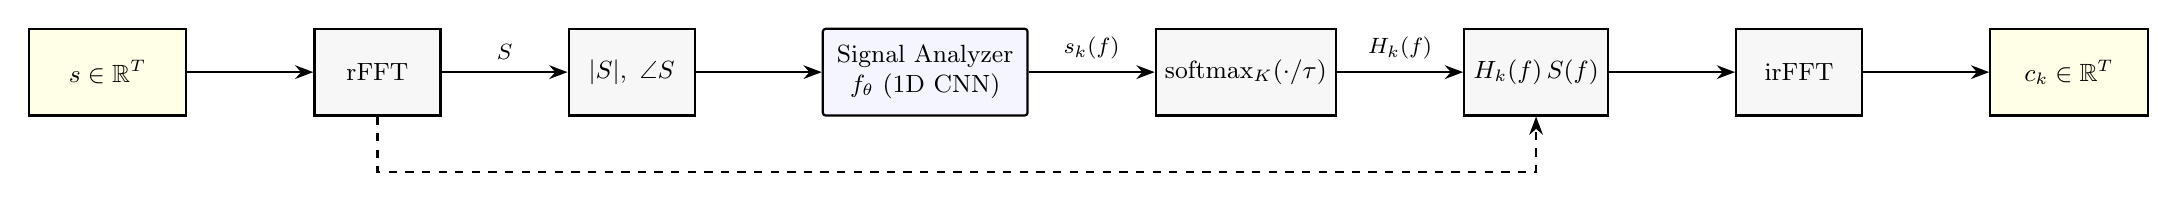
\begin{tikzpicture}[>=Stealth, node distance=14mm and 16mm,
  every node/.style = {font=\small},
  block/.style  = {rectangle, draw, thick, rounded corners=1pt,
                   minimum height=11mm, minimum width=26mm,
                   align=center, fill=blue!4},
  op/.style     = {rectangle, draw, thick, minimum height=11mm,
                   minimum width=16mm, align=center, fill=gray!6},
  io/.style     = {rectangle, draw, thick, minimum height=11mm,
                   minimum width=20mm, align=center, fill=yellow!10},
  arrow/.style  = {->, thick},
]
  \node[io] (sig) {$s\in\R^{T}$};
  \node[op, right=of sig] (fft) {$\rFFT$};
  \node[op, right=of fft] (magph)
    {$\lvert S\rvert,\ \angle S$};
  \node[block, right=of magph] (analyzer)
    {Signal Analyzer\\$f_{\theta}$~(1D CNN)};
  \node[op, right=of analyzer] (softmax)
    {$\softmax_{K}(\cdot/\tau)$};
  \node[op, right=of softmax] (prod)
    {$H_{k}(f)\,S(f)$};
  \node[op, right=of prod] (ifft) {$\irFFT$};
  \node[io, right=of ifft] (out) {$c_{k}\in\R^{T}$};

  \draw[arrow] (sig) -- (fft);
  \draw[arrow] (fft) -- node[above=1pt, font=\footnotesize]{$S$} (magph);
  \draw[arrow] (magph) -- (analyzer);
  \draw[arrow] (analyzer)
    -- node[above=1pt, font=\footnotesize]{$s_{k}(f)$} (softmax);
  \draw[arrow] (softmax)
    -- node[above=1pt, font=\footnotesize]{$H_{k}(f)$} (prod);
  \draw[arrow] (prod) -- (ifft);
  \draw[arrow] (ifft) -- (out);

  % Dashed bypass: S from rFFT output goes back to the multiplier
  \draw[arrow, dashed]
    (fft.south) -- ++(0,-7mm) -| (prod.south);
\end{tikzpicture}}
\caption{Architecture of NAFB. A 1D CNN analyzer reads the magnitude
and phase of the input spectrum $S=\rFFT(s)$ and predicts $K$
log-filter responses $s_{k}(f)$. A softmax over the $K$ dimension
produces non-negative filter weights $H_{k}(f)$ that sum to one at
every frequency bin (partition of unity). Each filter is multiplied
with the complex spectrum (dashed bypass) and inverse-transformed to
yield an IMF. The forward pass contains no unexplained operations.}
\label{fig:arch}
\end{figure*}

\paragraph{Signal analyzer.}
The analyzer $f_{\theta}$ is a small one-dimensional convolutional
network that operates on the $N$ frequency bins as spatial positions.
Its input is a two-channel spectrogram of the magnitude and phase of
$S$,
\begin{equation}
\bigl[\lvert S(f)\rvert,\ \angle S(f)\bigr] \in \R^{2 \times N} ,
\end{equation}
and its output is a stack of $K$ real-valued log-responses
$s_{k}(f) \in \R^{K \times N}$:
\begin{equation}
\bigl(s_{1}(f), \ldots, s_{K}(f)\bigr) \;=\; f_{\theta}\!\bigl(
\lvert S\rvert,\ \angle S\bigr) .
\label{eq:analyzer}
\end{equation}
The default configuration has an input $1\times 7$ convolution lifting
the two channels to $d=64$ hidden channels, three residual blocks of
two $1\times 5$ convolutions with batch normalisation and GELU
activations, and a $1\times 1$ output convolution projecting to $K$
channels. The total parameter count is $125{,}315$ for $K=3$.

\paragraph{Frequency partition.}
Per-frequency filter responses are obtained from a temperature-scaled
softmax across the $K$ dimension,
\begin{equation}
H_{k}(f) \;=\;
\frac{\exp\!\bigl(s_{k}(f)/\tau\bigr)}%
{\sum_{j=1}^{K}\exp\!\bigl(s_{j}(f)/\tau\bigr)} ,
\qquad \tau > 0 ,
\label{eq:softmax-partition}
\end{equation}
so that at every bin $f$ the $K$ filter weights are non-negative and
sum to one. The temperature $\tau$ controls filter sharpness: as
$\tau \to 0^{+}$, each $H_{k}(f)$ tends to an indicator of the highest
log-response, producing a disjoint partition of the frequency axis;
large $\tau$ gives broader, smoother filters. We anneal $\tau$ during
training (Section~\ref{subsec:training}).

\paragraph{IMF extraction.}
The $K$ IMFs are obtained by pointwise multiplication of the filters
with the complex spectrum, followed by the inverse real FFT at length
$T$:
\begin{equation}
c_{k} \;=\; \irFFT_{T}\!\bigl(H_{k}(f)\,S(f)\bigr) .
\label{eq:imf}
\end{equation}
The entire pipeline is differentiable with respect to the analyzer
parameters $\theta$, so the decomposition can be trained jointly with
any downstream differentiable loss (Section~\ref{sec:taskaware}).

\begin{remark}[Length-agnostic operation]
The analyzer is a fully-convolutional 1D network over frequency bins;
no fixed length is baked into its weights. A model trained at signal
length $T$ can be applied at any other length $T'$ (and any sample
rate) with no modification, since $\lvert S\rvert$ and $\angle S$ are
the only inputs. The trained checkpoint (optimised at $T = 512$,
$f_{s} = 512$ Hz) was evaluated on $200$ in-distribution AM--FM
composites at each of $T \in \{256, 512, 1024, 2048, 4096\}$ with
$f_{s} = 512$ Hz: orthogonality index $\mathrm{OI} \leq 0.004$ and
energy ratio $\mathrm{ER} = 1.000 \pm 0.000$ at every length, with
per-signal inference $\approx 4$\,ms on MPS. The architectural
guarantees hold unchanged at inference lengths up to $8\times$ the
training length.
\end{remark}

\begin{remark}[Phase channel]
Including the phase $\angle S$ alongside $\lvert S\rvert$ lets the
analyzer distinguish signals with identical power spectra but
different temporal structure (e.g., a steady tone vs.\ a matched-energy
chirp). A magnitude-only ablation is a natural future check.
\end{remark}

\begin{remark}[On the name \emph{NAFB}]
The mechanism here is a one-shot global filter bank, not EMD's
iterative envelope sifting. We retain the EMD framing because (i) EMD
was itself characterised as an adaptive filter bank on stochastic
input~\cite{flandrin2004emdfilterbank}, so the interpretive role of
an IMF as a narrow-band oscillatory component is the role our filters
produce, and (ii) the output shape (ordered bandpass components) is
the one classical-EMD users already know how to read. Readers who
prefer a mechanism-level name may read the contribution as a
\emph{neural adaptive filter bank with exact reconstruction by identity}; nothing
in the theory or experiments depends on the label.
\end{remark}

% ---------------------------------------------------------------------
\subsection{Architectural Guarantees}
\label{subsec:theory}

We now state the three properties that hold for NAFB by construction,
independent of any loss or training procedure. All three follow from a
single algebraic fact --- that the softmax output in~\eqref{eq:softmax-partition}
is a non-negative partition of unity over $K$ elements --- combined with
the linearity of the inverse FFT and Parseval's identity.

\begin{proposition}[Exact reconstruction]
\label{prop:recon}
For any input signal $s \in \R^{T}$, any temperature $\tau > 0$, and
any analyzer output $s_{k}(f) \in \R^{K\times N}$, the components
defined by~\eqref{eq:imf} satisfy
\begin{equation}
\sum_{k=1}^{K} c_{k}(t) \;=\; s(t), \qquad t = 0, 1, \ldots, T-1 ,
\end{equation}
with equality exact up to the floating-point round-off of the
$\rFFT$ / $\irFFT$ pair.
\end{proposition}

\begin{proof}
By linearity of the inverse FFT and~\eqref{eq:softmax-partition},
\[
\sum_{k=1}^{K} c_{k}
= \irFFT_{T}\!\Bigl(\Bigl(\sum_{k=1}^{K} H_{k}(f)\Bigr) S(f)\Bigr)
= \irFFT_{T}(S(f)) = s ,
\]
where the penultimate equality uses $\sum_{k} H_{k}(f) = 1$ at every
$f$ and the last uses that $\irFFT_{T}$ inverts $\rFFT$ on real
signals of length $T$.
\end{proof}

\begin{proposition}[Energy boundedness]
\label{prop:energy}
For any input $s$,
\begin{equation}
\sum_{k=1}^{K} \|c_{k}\|_{2}^{2} \;\leq\; \|s\|_{2}^{2} ,
\label{eq:energy-bound}
\end{equation}
with equality if and only if the filters form a disjoint partition,
i.e.\ for each $f$ there is some $k(f)$ with $H_{k(f)}(f)=1$ and
$H_{j}(f)=0$ for $j\neq k(f)$.
\end{proposition}

\begin{proof}
By Parseval's identity and~\eqref{eq:imf},
$\|c_{k}\|_{2}^{2}$ equals (up to a constant depending on the FFT
normalisation) $\sum_{f} H_{k}(f)^{2} \lvert S(f)\rvert^{2}$.
Summing over $k$ and exchanging the order of summation,
\begin{equation}
\sum_{k=1}^{K} \|c_{k}\|_{2}^{2}
= \sum_{f} \lvert S(f)\rvert^{2} \sum_{k=1}^{K} H_{k}(f)^{2} .
\label{eq:parseval-sum}
\end{equation}
Since $H_{k}(f) \in [0,1]$ and $\sum_{k} H_{k}(f) = 1$, the Cauchy--Schwarz
inequality (equivalently, the power-mean inequality) gives
$\sum_{k} H_{k}(f)^{2} \leq \bigl(\sum_{k} H_{k}(f)\bigr)^{2} = 1$,
with equality iff the vector $\bigl(H_{1}(f), \ldots, H_{K}(f)\bigr)$
is a standard basis vector. The result follows from Parseval once more,
$\sum_{f} \lvert S(f)\rvert^{2} = \|s\|_{2}^{2}$.
\end{proof}

\begin{proposition}[Non-negativity and bandpass interpretation]
\label{prop:nonneg}
For any input, any temperature $\tau > 0$, and any $(k,f)$ the filter
response satisfies $H_{k}(f) \geq 0$. Consequently, each IMF $c_{k}$
is a bandpass-filtered version of $s$ obtained by multiplying the
spectrum $S(f)$ by a non-negative, per-bin attenuation
$H_{k}(f) \in [0,1]$.
\end{proposition}

\begin{proof}
$H_{k}(f)$ is the $k$-th component of a softmax output, hence a
probability in $[0,1]$; $\sum_{k} H_{k}(f) = 1$ was shown in
Proposition~\ref{prop:recon}. Equation~\eqref{eq:imf} is the inverse
transform of $S(f)$ modulated by $H_{k}(f) \in [0,1]$, which is the
definition of a linear bandpass filter with real, non-negative
frequency response.
\end{proof}

Propositions~\ref{prop:recon}--\ref{prop:nonneg} are stated without any
assumption on the analyzer: they hold at initialisation, during
training, and at inference, on any input signal, with any $K$ and any
$\tau > 0$. They are the structural counterpart of the soft constraints
(reconstruction loss, energy-conservation loss, non-negativity penalty)
that physics-informed approaches typically add to the training
objective. Because they are enforced by the parameterisation itself,
the training loss need not contain any term for them. We return to this
point in Section~\ref{sec:negative-result}.

\begin{corollary}[Approximate orthogonality]
\label{cor:ortho}
For any two IMFs $c_{k}$ and $c_{\ell}$ with $k \neq \ell$,
\begin{equation}
\lvert \langle c_{k}, c_{\ell} \rangle \rvert \;\leq\;
\sum_{f} H_{k}(f)\, H_{\ell}(f)\, \lvert S(f)\rvert^{2} .
\end{equation}
In particular, if $H_{k}$ and $H_{\ell}$ have disjoint support on the
frequency axis, then $\langle c_{k}, c_{\ell}\rangle = 0$.
\end{corollary}

\begin{proof}
By Parseval,
$\langle c_{k}, c_{\ell}\rangle =
\sum_{f} H_{k}(f) H_{\ell}(f) \lvert S(f)\rvert^{2}$ (up to the FFT
normalisation), and every summand is non-negative by
Proposition~\ref{prop:nonneg}. Disjoint support makes every summand
zero.
\end{proof}

As $\tau \to 0^{+}$ the softmax partition becomes the argmax indicator;
supports become disjoint and Corollary~\ref{cor:ortho} makes the cross
terms exactly zero. At finite $\tau$, the bound on overlap is governed
by the signal-weighted product of adjacent filters. In
Section~\ref{sec:experiments} we report measured orthogonality indices
of $0.00 \pm 0.01$ across five test distributions, compared with
$0.04$--$0.10$ for EMD and VMD.

% ---------------------------------------------------------------------
\subsection{Training Losses}
\label{subsec:loss}

Because Propositions~\ref{prop:recon}--\ref{prop:nonneg} relieve the
loss of the reconstruction/energy-conservation duties, the training
objective reduces to four terms that shape the \emph{quality} of the
decomposition rather than its feasibility:
\begin{equation}
\begin{split}
\mathcal{L} \;=\;&
 \lambda_{\mathrm{sharp}}\,\mathcal{L}_{\mathrm{sharp}}
+\lambda_{\mathrm{order}}\,\mathcal{L}_{\mathrm{order}}
+\lambda_{\mathrm{ortho}}\,\mathcal{L}_{\mathrm{ortho}} \\
&+\lambda_{\mathrm{bal}}\,\mathcal{L}_{\mathrm{bal}}
+\lambda_{\mathrm{task}}\,\mathcal{L}_{\mathrm{task}} .
\end{split}
\label{eq:total-loss}
\end{equation}
The first four are always present; the task term is optional and only
activates for end-to-end training (Section~\ref{sec:taskaware}).
Default weights are $\lambda_{\mathrm{sharp}}=2$,
$\lambda_{\mathrm{order}}=2$, $\lambda_{\mathrm{ortho}}=0.1$,
$\lambda_{\mathrm{bal}}=5$; we use these throughout.

\paragraph{Signal-weighted sharpness.}
A broad, flat filter $H_{k}(f) \approx 1/K$ is a valid partition of
unity (summing to one with zero entropy contribution per bin) but
corresponds to no decomposition at all. We penalise the signal-weighted
Shannon entropy of each filter,
\begin{equation}
\mathcal{L}_{\mathrm{sharp}} \;=\; \frac{1}{K\log N}
  \sum_{k=1}^{K}
  \mathrm{H}\!\bigl(p_{k}\bigr),
\label{eq:sharp}
\end{equation}
with $p_{k}(f) = H_{k}(f)\lvert S(f)\rvert^{2}
  / \sum_{f'} H_{k}(f')\lvert S(f')\rvert^{2}$ the
signal-weighted filter density.
so that filters that isolate a narrow band of \emph{signal} energy are
rewarded, but no penalty is applied to broad-but-silent frequency
regions. This term is essential: without it, the network satisfies
every remaining constraint by choosing $H_{k}(f) = 1/K$ everywhere.

\paragraph{Centroid separation.}
For each IMF we compute the signal-weighted spectral centroid
$\bar{f}_{k}$ and normalise it to the Nyquist range,
$\hat{f}_{k} = \bar{f}_{k}/\Nyq \in [0,1]$. The centroid-separation
loss combines three terms (ordering, repulsion, coverage):
\begin{align}
\mathcal{L}_{\mathrm{order}} \;=\;
 \frac{1}{K-1}\sum_{k=1}^{K-1}
   \bigl[\max(0, \hat{f}_{k+1} - \hat{f}_{k} + m)\bigr]^{2} \nonumber\\
-\frac{\eta_{r}}{K(K-1)}\sum_{i \neq j}
    \log\!\bigl(\lvert\hat{f}_{i} - \hat{f}_{j}\rvert + \epsilon\bigr)
-\eta_{c}\,\mathrm{Var}\!\bigl(\hat{f}_{1},\ldots,\hat{f}_{K}\bigr) .
\label{eq:order}
\end{align}
The first (squared hinge, margin $m = 0.02$) enforces descending
centroids; the second is a pairwise log-distance repulsion that acts on
all pairs, not only consecutive ones; the third rewards coverage of the
Nyquist axis via centroid variance. Each of these terms addresses a
distinct failure mode discovered during development
(Section~\ref{sec:negative-result}); the full ablation is in
Appendix~\ref{app:ablation}. Default sub-weights are $\eta_{r}=0.5$,
$\eta_{c}=0.3$ and $\epsilon=10^{-4}$.

\paragraph{Soft orthogonality.}
Although Corollary~\ref{cor:ortho} already gives near-orthogonality at
small $\tau$, a mild soft penalty on the cosine similarity between IMF
pairs accelerates training:
\begin{equation}
\mathcal{L}_{\mathrm{ortho}} \;=\; \frac{1}{K(K-1)}
  \sum_{i\neq j}
  \Bigl(\tfrac{\langle c_{i}, c_{j}\rangle}
              {\|c_{i}\|_{2}\,\|c_{j}\|_{2} + \epsilon}\Bigr)^{2} .
\label{eq:ortho}
\end{equation}
Its weight $\lambda_{\mathrm{ortho}} = 0.1$ is small; in the trained
model the measured orthogonality index is at the $10^{-4}$ level.

\paragraph{Filter balance.}
The softmax partition admits a degenerate solution in which one filter
covers the whole axis and the remaining $K{-}1$ are zero; this is a
valid partition of unity but a useless decomposition. The balance loss
requires each filter to cover at least a minimum fraction of the
frequency axis on average:
\begin{equation}
\mathcal{L}_{\mathrm{bal}} \;=\; \frac{1}{K}
  \sum_{k=1}^{K}
  \max\!\bigl(0,\ \alpha - \overline{H_{k}}\bigr),\qquad
\overline{H_{k}} = \frac{1}{N}\sum_{f} H_{k}(f) ,
\label{eq:balance}
\end{equation}
with $\alpha = 1/(2K)$. With $K=3$, each filter must cover at least one
sixth of the axis on average; a filter that disappears entirely incurs
a maximal penalty.

% ---------------------------------------------------------------------
\subsection{Training Procedure}
\label{subsec:training}

\paragraph{Data.}
We train on synthetic AM--FM composites of 2--3 mono-components drawn
uniformly from three frequency bands ($40$--$100$ Hz, $10$--$30$ Hz,
and $1$--$8$ Hz at $T=512$, $f_{s}=512$ Hz), modulated with random
amplitude and frequency envelopes, and corrupted with additive Gaussian
noise at SNR in $[10, 40]$ dB. The training set contains $2000$
signals; the validation set $200$. Generation is online and seeded, so
no fixed dataset is required to reproduce training.

\paragraph{Temperature annealing.}
The softmax temperature is annealed linearly from $\tau_{0} = 2.0$ down
to $\tau_{\mathrm{end}} = 0.3$ over the first $40$ epochs, then held
constant. The warm start gives well-conditioned gradients over the
whole partition; the low final temperature yields near-disjoint filters
at inference, making Proposition~\ref{prop:energy}'s bound tight and
Corollary~\ref{cor:ortho}'s cross-terms negligible.

\paragraph{Optimisation.}
We use Adam~\cite{kingma2015adam} with learning rate $10^{-3}$, weight
decay $10^{-4}$, gradient-norm clipping at $1.0$, and a cosine
learning-rate schedule over $100$ epochs. Batch size is $32$. All
training runs on CPU; no GPU is required. A full training run of the
default $K=3$, $d=64$ model takes approximately $45$ minutes on six
CPU cores.

% ---------------------------------------------------------------------
\subsection{Inference-Time IMF Ordering}
\label{subsec:sort}

For downstream consumption it is convenient to order IMFs in a fixed
convention --- classically, by descending frequency. After the forward
pass~\eqref{eq:imf} we compute the signal-weighted centroid
\begin{equation}
\bar{f}_{k} \;=\;
\frac{\sum_{f} f\,H_{k}(f)\lvert S(f)\rvert^{2}}
      {\sum_{f} H_{k}(f)\lvert S(f)\rvert^{2}}
\end{equation}
and permute the $K$ IMFs in descending order of $\bar{f}_{k}$. The
operation is a pure permutation, so it preserves every structural
property (reconstruction, partition of unity, energy bound, and
orthogonality) exactly. At training time the permutation is disabled so
the ordering loss sees raw model output.

\paragraph{Canonical decomposition example.}
Figure~\ref{fig:canonical} shows the learned filter responses and the
corresponding decomposition on a canonical three-component signal
(dominant frequencies at $50$, $15$, and $3$ Hz; $T=1024$, $f_{s}=1000$
Hz). The three softmax filters form a clean bandpass partition of the
Nyquist axis, and each IMF is concentrated around its assigned band.

\begin{figure}[t]
\centering
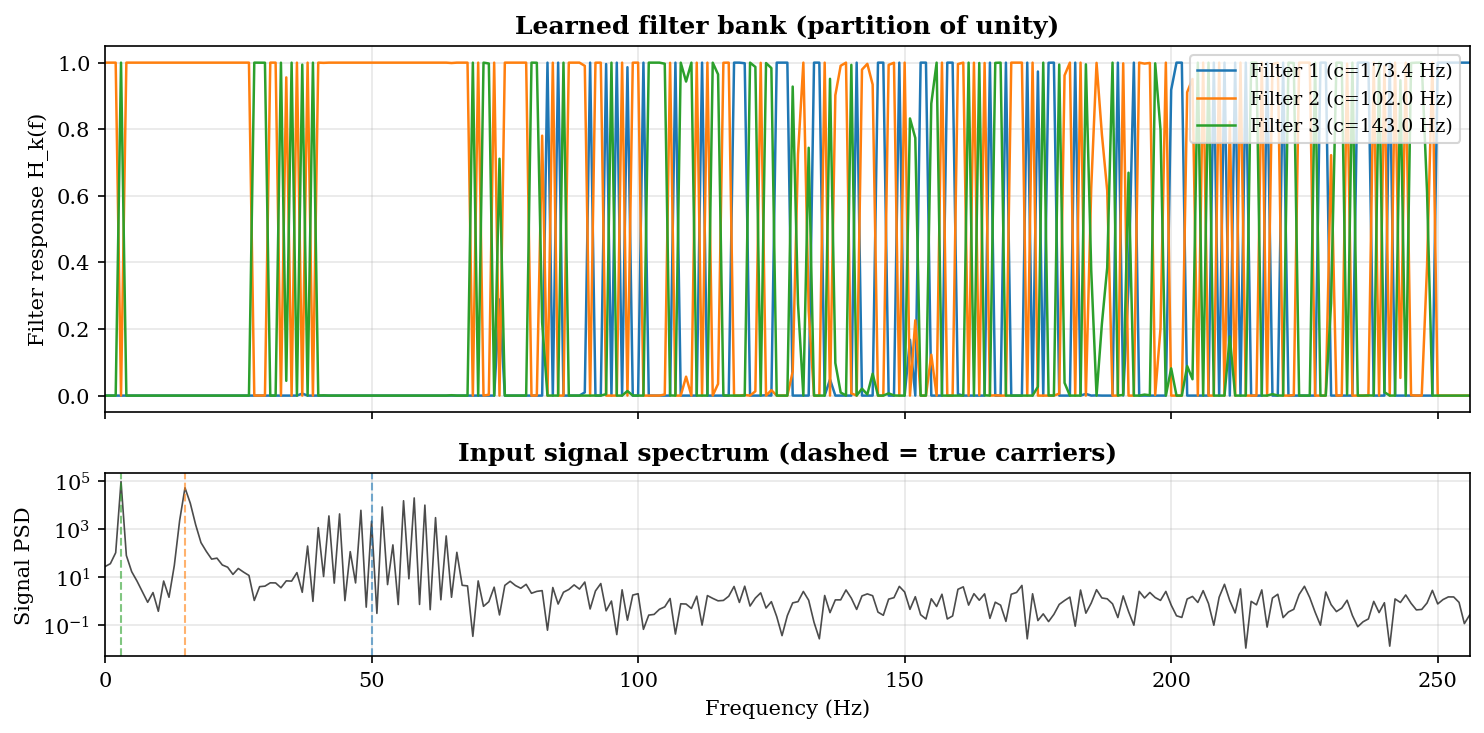
\includegraphics[width=\columnwidth]{figs/filters_canonical.png}
\caption{Learned softmax filter responses $H_{k}(f)$ on the canonical
three-component signal. The three filters partition the Nyquist axis
into disjoint-in-practice bandpass regions; their sum equals one at
every bin by construction (Proposition~\ref{prop:recon}).}
\label{fig:canonical}
\end{figure}

% =====================================================================
\section{The Case for Architectural Inductive Bias}
\label{sec:negative-result}
% =====================================================================

The architecture of Section~\ref{sec:method} is a non-obvious choice.
A more direct route --- the one we took first --- is to replicate
EMD's sifting structure with a neural operator and to shape the
decomposition through soft physics losses on orthogonality, bandwidth,
energy, and ordering. That route failed, in informative ways. This
section documents the failure, because the lesson generalises beyond
our setting: soft physics constraints are necessary but do not
uniquely specify a decomposition, and iteratively adding penalties
does not shrink the feasible set --- it relocates the optimiser to a
new degenerate minimum. Architectural constraints do shrink the
feasible set.

% ---------------------------------------------------------------------
\subsection{Iterative Neural Sifting}
\label{subsec:sifting}

Our first prototype mirrored EMD's sequential structure. Let $g_{\phi}$
be a learned sifting operator. Given the current residual $r_{k-1}$
and the IMF index $k$, it extracts one IMF,
\begin{equation}
c_{k} \;=\; g_{\phi}(r_{k-1},\, k) ,
\qquad
r_{k} \;=\; r_{k-1} - c_{k} ,
\label{eq:sifting}
\end{equation}
with $r_{0} = s$. After $K$ iterations the reconstruction
$s = \sum_{k} c_{k} + r_{K}$ holds exactly, since $r_{K}$ is defined
by the subtraction recurrence. The remaining properties
(bandpass concentration, orthogonality, energy conservation, ordering)
must be induced by the loss.

The operator $g_{\phi}$ is a FiLM-conditioned one-dimensional U-Net:
a three-level encoder with max-pooling, a bottleneck, a symmetric
decoder with skip connections, and a $1{\times}1$ output projection.
The IMF index $k$ is embedded in a learned lookup and passed through
a FiLM generator~\cite{perez2018film} that produces per-channel
$(\gamma, \beta)$ modulation parameters at every block. A bandpass
prior, implemented as $K$ learnable windowed-sinc filters initialised
to cover distinct frequency bands, is concatenated with the signal as
an auxiliary input channel to break the symmetry that would otherwise
make all IMF indices interchangeable at initialisation. The network
has roughly $3{\times}10^{5}$ parameters at our default configuration.

This is a generic, expressive function approximator, and a reasonable
one on paper. It can in principle reproduce EMD, VMD, or any other
decomposition for which the $K$-step sifting structure is appropriate.

% ---------------------------------------------------------------------
\subsection{Seven Soft Physics Losses}
\label{subsec:sifting-loss}

Without a per-frequency partition of unity to enforce the four target
properties, each property needs a loss. Our seven-term objective was
\begin{equation}
\mathcal{L}^{\text{sift}} \;=\; \sum_{i \in \mathcal{I}}
  \lambda_{i}\,\mathcal{L}_{i} ,
\label{eq:sifting-loss}
\end{equation}
with index set $\mathcal{I}$ containing the seven components listed in
Table~\ref{tab:sifting-losses}. The table is not an ablation of the
final design; it is a chronological record of what was added, in
response to what failure.

\begin{table}[t]
\centering
\caption{The seven-term sifting loss. Each row corresponds to one
property and one historical addition; the next failure row names the
degenerate solution the optimiser found once the property was
enforced.}
\label{tab:sifting-losses}
\setlength{\tabcolsep}{3pt}
\begin{tabular}{@{}p{0.18\columnwidth}p{0.32\columnwidth}p{0.40\columnwidth}@{}}
\toprule
Loss            & Target property                     & Subsequent failure mode \\
\midrule
ortho           & cross-correlation $\langle c_{i}, c_{j}\rangle\!=\!0$ &
                  trivial residual ($c_{k}\!\equiv\!0$) \\
narrow          & low spectral bandwidth per IMF       &
                  (same; zero-bandwidth IMFs are trivial)\\
res             & $\|r_{K}\|^{2}$ small                 &
                  energy inflation ($\Sigma\|c_{k}\|^{2}\!>\!\|s\|^{2}$)\\
cons            & Parseval: $\Sigma\|c_{k}\|^{2}\!+\!\|r_{K}\|^{2}\!=\!\|s\|^{2}$ &
                  degenerate centroid clustering \\
order           & descending spectral centroids        &
                  empty-spectrum centroids \\
mono            & monotonic residual ($\dot r\!>\!0$)      &
                  (orthogonal to spectral failures) \\
conc            & low spectral entropy per IMF           &
                  same clustering as centroid failures \\
\bottomrule
\end{tabular}
\end{table}

% ---------------------------------------------------------------------
\subsection{Four Failure Modes}
\label{subsec:failures}

Each row of Table~\ref{tab:sifting-losses} was added to close a
specific hole. Each one, in turn, exposed a new hole. The pattern
repeats four times.

\paragraph{F1: Trivial residual.}
With only orthogonality and narrow-band losses active, the global
minimum is the trivial solution
$c_{1} = \cdots = c_{K} = 0$, $r_{K} = s$. Zero IMFs are trivially
orthogonal and trivially narrow-band, and the sifting recurrence does
not penalise energy left in the residual. The reconstruction identity
holds; no decomposition occurs.

\paragraph{F2: Energy inflation.}
Adding $\mathcal{L}_{\mathrm{res}}$ (residual-energy penalty) closes
F1 but opens a new door. The optimiser now finds IMFs whose total
energy exceeds the signal's, with the excess cancelled by negative
cross-correlations among the components. On the canonical
three-component test signal we measured
$\sum_{k}\|c_{k}\|_{2}^{2} \approx 4.17\,\|s\|_{2}^{2}$, and the
cosine-similarity orthogonality loss was still low because the
pairwise products of these mutually-cancelling components happened to
fall near zero. The reconstruction identity still holds, but the
individual IMFs have no physical meaning.

\paragraph{F3: Degenerate ordering.}
Adding $\mathcal{L}_{\mathrm{cons}}$ (Parseval energy conservation)
closes F2. The optimiser now finds IMFs whose centroids
$(\bar{f}_{1}, \bar{f}_{2}, \bar{f}_{3}) = (35.7,\ 3.2,\ 3.1)$ Hz on
a signal with true components at $(50,\ 15,\ 3)$ Hz. Ordering is
technically satisfied (the centroids are weakly descending), but IMF~1
absorbs both high-frequency components, IMFs~2 and~3 split the lowest
component, and the middle frequency is unrepresented. The
frequency-ordering hinge gives no gradient once adjacent centroids are
more than the margin apart, even if they sit on top of each other.

\paragraph{F4: Empty spectrum.}
Adding a centroid-repulsion term to $\mathcal{L}_{\mathrm{order}}$
closes F3 --- centroids now spread. But the optimiser promptly relocates
one filter to a region with no signal energy:
$(\bar{f}_{1}, \bar{f}_{2}, \bar{f}_{3}) = (174.6,\ 35.7,\ 3.1)$ Hz,
with IMF~1 sitting at a frequency near the Nyquist limit where the
signal has essentially no power. All constraints are now satisfied
(ordering, repulsion, energy conservation, orthogonality,
narrow-band), yet the mode-mixing metric on the target bands
($50$, $15$, $3$ Hz) is no better than the F3 solution.

Across these four iterations we added twelve sub-parameters and two
months of tuning, and the training runs kept finding new degenerate
solutions faster than we could write losses for them. The difficulty
is not a tuning problem. It is structural.

% ---------------------------------------------------------------------
\subsection{Diagnosis: Soft Constraints Do Not Shrink the Feasible Set}
\label{subsec:diagnosis}

Each soft-constraint loss $\mathcal{L}_{i}$ penalises deviation from
some property; it does not forbid it. Minimisers of~\eqref{eq:sifting-loss}
achieve small but non-zero values of every $\mathcal{L}_{i}$ and trade
the residual error in one term against slack in another. In a
high-capacity function class like a U-Net, the optimiser has enormous
freedom to find points that satisfy every loss to first order without
satisfying any of them in a physically meaningful way.

This is the standard story of constrained optimisation under
penalty-method reformulation. If the feasible set is defined only
through penalties, it is not the set the penalties describe; it is
whichever sub-level set of the Lagrangian the optimiser settles into.
In a convex setting with well-chosen multipliers, those sub-level sets
approach the feasible set as the multipliers grow. In a non-convex
setting with a finite multiplier budget, they do not --- and the
optimiser is free to exploit the slack. Every row of
Table~\ref{tab:sifting-losses} is a symptom of that slack.

The architecture of Section~\ref{sec:method} does not add to the
penalties. It changes the parameterisation so that the sought
properties are consequences of the forward pass rather than targets of
the loss:
\begin{itemize}
\item Trivial residual (F1) is impossible: the residual $r_{K}$ is
  identically zero by Proposition~\ref{prop:recon}.
\item Energy inflation (F2) is impossible:
  Proposition~\ref{prop:energy} bounds $\sum_{k}\|c_{k}\|_{2}^{2}$
  above by $\|s\|_{2}^{2}$.
\item Degenerate ordering (F3) is eliminated by the
  centroid-separation loss combined with the signal-weighted sharpness
  loss, which together reshape the gradient field so that the
  optimiser can only satisfy them by spreading centroids across
  populated spectrum.
\item Empty-spectrum placements (F4) are prevented by the filter
  balance loss~\eqref{eq:balance}: a filter that vacates the spectrum
  has zero average coverage and incurs a maximal penalty.
\end{itemize}

The first two are structural guarantees (Propositions~\ref{prop:recon}
and~\ref{prop:energy}). The second two require loss terms, but those
losses now operate in a one-dimensional quantity (the filter profile
$H_{k}(f)$ over $N$ bins) whose feasible set is already restricted to
non-negative functions summing to one.

\begin{remark}[Scope of the lesson]
The failure mode is not specific to signal decomposition. Any
physics-informed learning setting in which multiple intertwined
properties are enforced by soft penalties --- PINN-type problems with
boundary conditions, constrained generative models, symmetry-preserving
networks --- is susceptible to the same structural slack. Where
possible, it is better to parameterise the feasible set directly.
\end{remark}

% =====================================================================
\section{Experiments}
\label{sec:experiments}
% =====================================================================

We evaluate NAFB on four axes. Section~\ref{subsec:decomp} demonstrates
decomposition quality on nonstationary synthetic signals.
Section~\ref{subsec:generalization} compares NAFB, VMD, and EMD on a
controlled 5-distribution generalization study.
Section~\ref{sec:taskaware} is the central experiment: task-aware
classification at three signal-to-noise ratios, showing where
end-to-end training wins and where it loses. Section~\ref{subsec:pupil}
extends the decomposition quality result to real biomedical data
(pupillometry). Section~\ref{subsec:cost} reports computational cost.

All experiments use the same trained analyzer checkpoint (the one
released with the repository), $K = 3$, $d = 64$ hidden channels,
three residual blocks --- the architecture of Section~\ref{sec:method}.
Baselines use standard reference implementations with $K = 3$ modes to
match: EMD via the \texttt{EMD-signal} library with its default sifting
parameters and VMD via \texttt{vmdpy} with penalty parameter
$\alpha = 2000$ and dual ascent step $\tau = 0$, both library defaults.

\subsection{Evaluation Metrics}
\label{subsec:metrics}

Three quantitative metrics appear throughout. For a set of $K$
components $\{c_{k}\}$ and the original signal $s$:

\emph{Orthogonality index (OI)}:
\begin{equation}
\mathrm{OI} \;=\;
 \frac{2\sum_{i < j} \lvert\langle c_{i}, c_{j}\rangle\rvert}%
      {\sum_{k}\|c_{k}\|_{2}^{2}} .
\label{eq:oi}
\end{equation}
A perfect orthogonal decomposition has $\mathrm{OI} = 0$.

\emph{Energy ratio}:
\begin{equation}
\mathrm{ER} \;=\;
 \frac{\sum_{k}\|c_{k}\|_{2}^{2}}{\|s\|_{2}^{2}} .
\label{eq:er}
\end{equation}
Parseval-type energy conservation corresponds to $\mathrm{ER} = 1$.
Values $>1$ indicate energy inflation; values $<1$ indicate signal
content lost to a residual or to destructive overlap.

\emph{Mode-mixing index (MMI)}: when ground-truth components
$\{g_{\ell}\}_{\ell = 1}^{L}$ are available (synthetic benchmarks),
assign each $g_{\ell}$ to its best-correlated estimated component and
report
\begin{equation}
\mathrm{MMI} \;=\;
 \frac{1}{L}\sum_{\ell=1}^{L}
 \left(
   1 - \max_{k}
   \frac{\lvert\langle g_{\ell}, c_{k}\rangle\rvert}
        {\|g_{\ell}\|_{2}\,\|c_{k}\|_{2}}
 \right) .
\label{eq:mmi}
\end{equation}
$\mathrm{MMI} \in [0, 1]$: zero means every ground-truth component is
recovered cleanly inside some IMF; one means no IMF correlates
appreciably with any ground-truth component. The metric is
assignment-based (each $g_{\ell}$ picks its best match), so two true
components mapping to the same IMF are penalised as mixing.

% ---------------------------------------------------------------------
\subsection{Decomposition Quality on Nonstationary Signals}
\label{subsec:decomp}

As a visual smoke test we run NAFB, EMD, and VMD on five classes of
nonstationary three-component composites: stationary AM--FM, piecewise
(amplitude step), a chirp trio (three simultaneous linear chirps at
separated frequency ranges), crossing chirps (two components that
sweep through each other in frequency), and widening AM (time-varying
bandwidth). Representative decompositions are in
Fig.~\ref{fig:nonstat-example}.

\begin{figure*}[t]
\centering
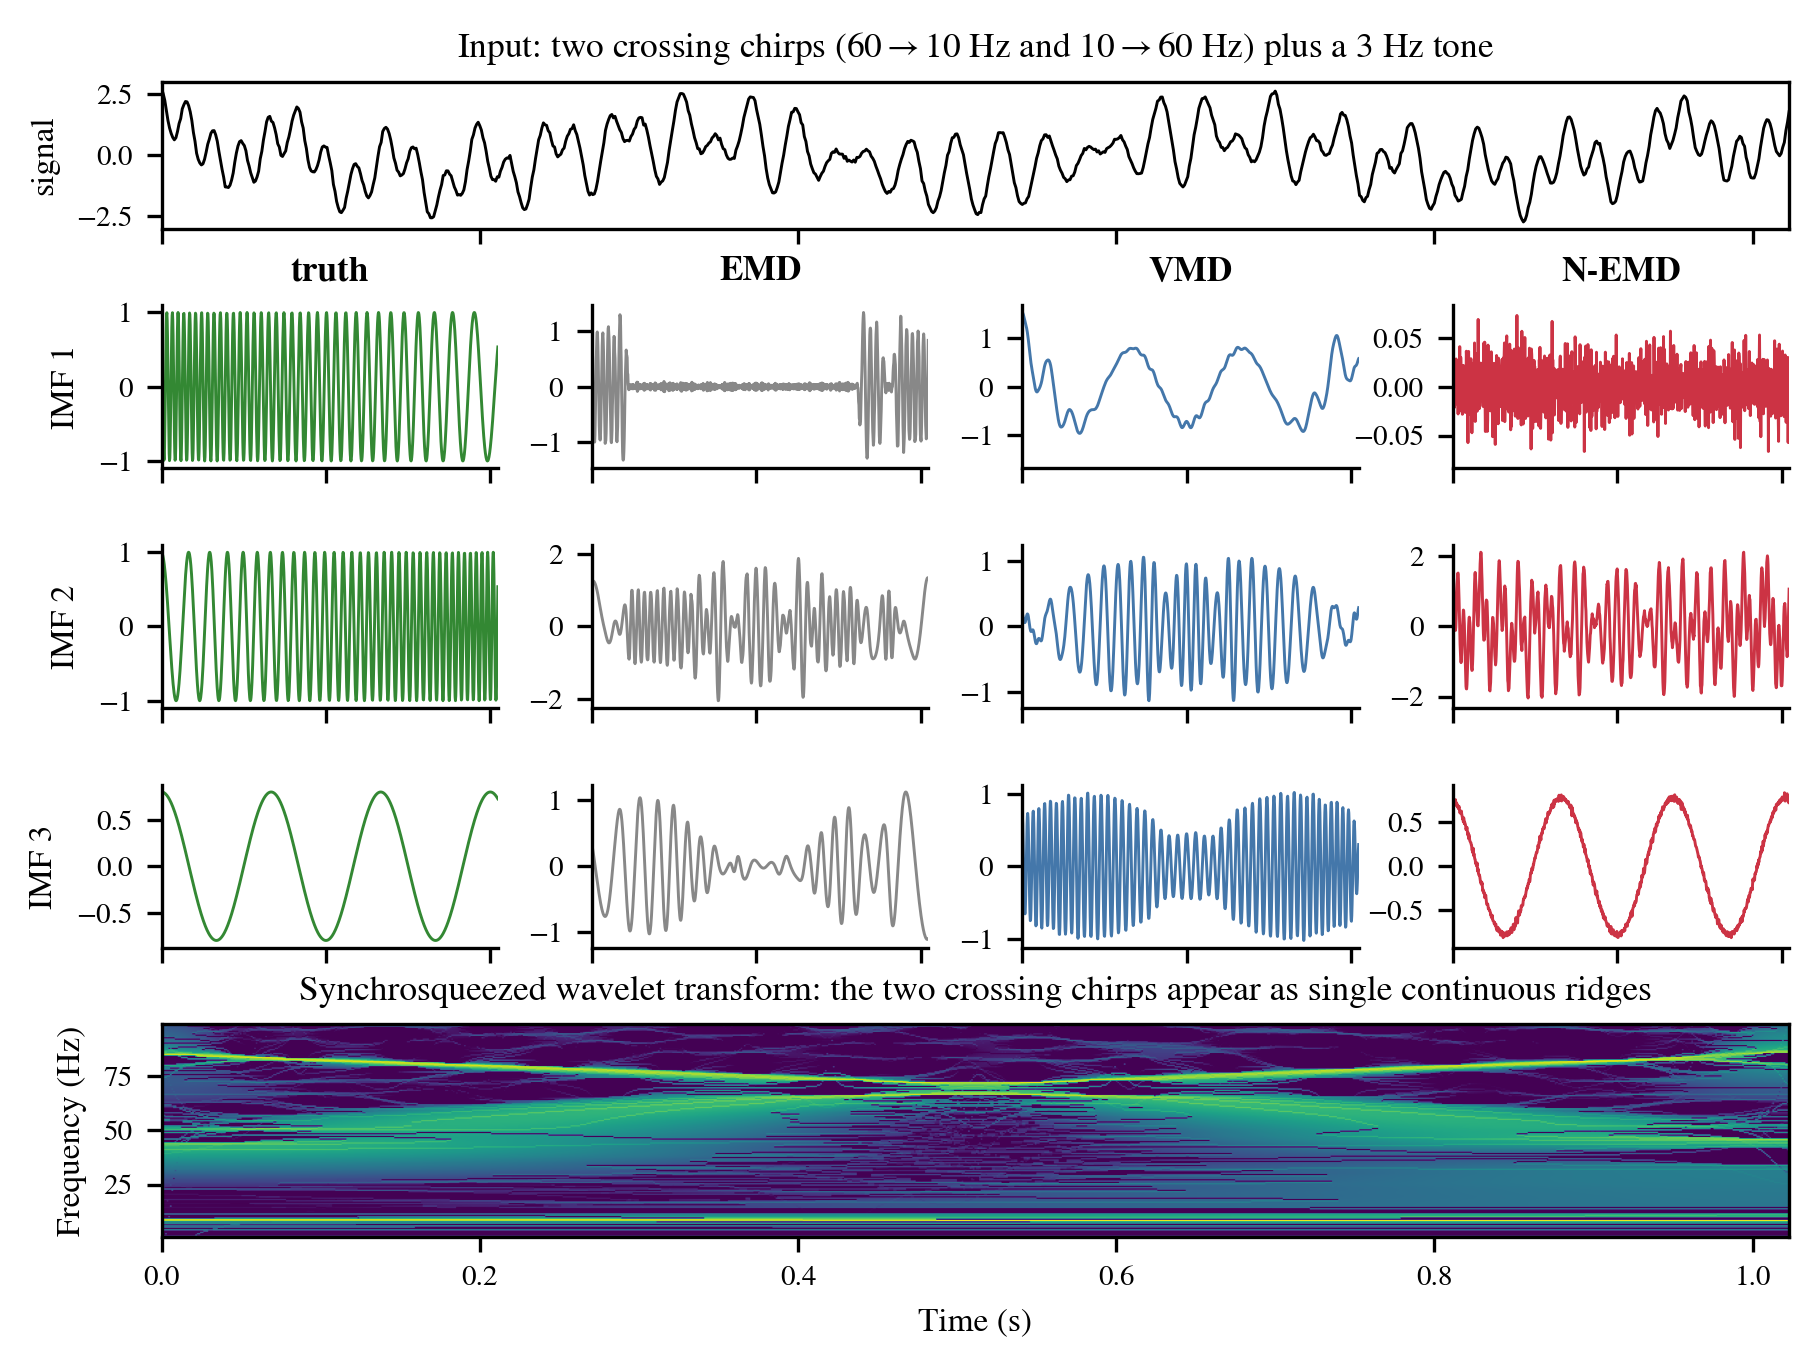
\includegraphics[width=0.85\textwidth]{figs/crossing_chirps_with_ssq.png}
\caption{Crossing-chirps benchmark. Top: a two-crossing-chirps signal
plus a $3$\,Hz tone. Middle rows: ground-truth components vs.\ IMFs from
EMD, VMD, and NAFB --- every frequency-partitioning decomposition
splits each chirp across bands. Bottom:
synchrosqueezed~\cite{daubechies2011synchrosqueezing} wavelet transform
of the same signal renders the chirps as single continuous ridges.
Decomposition and time-frequency ridge extraction answer different
questions; the paper claims the former, not the latter.}
\label{fig:nonstat-example}
\end{figure*}

\begin{figure*}[t]
\centering
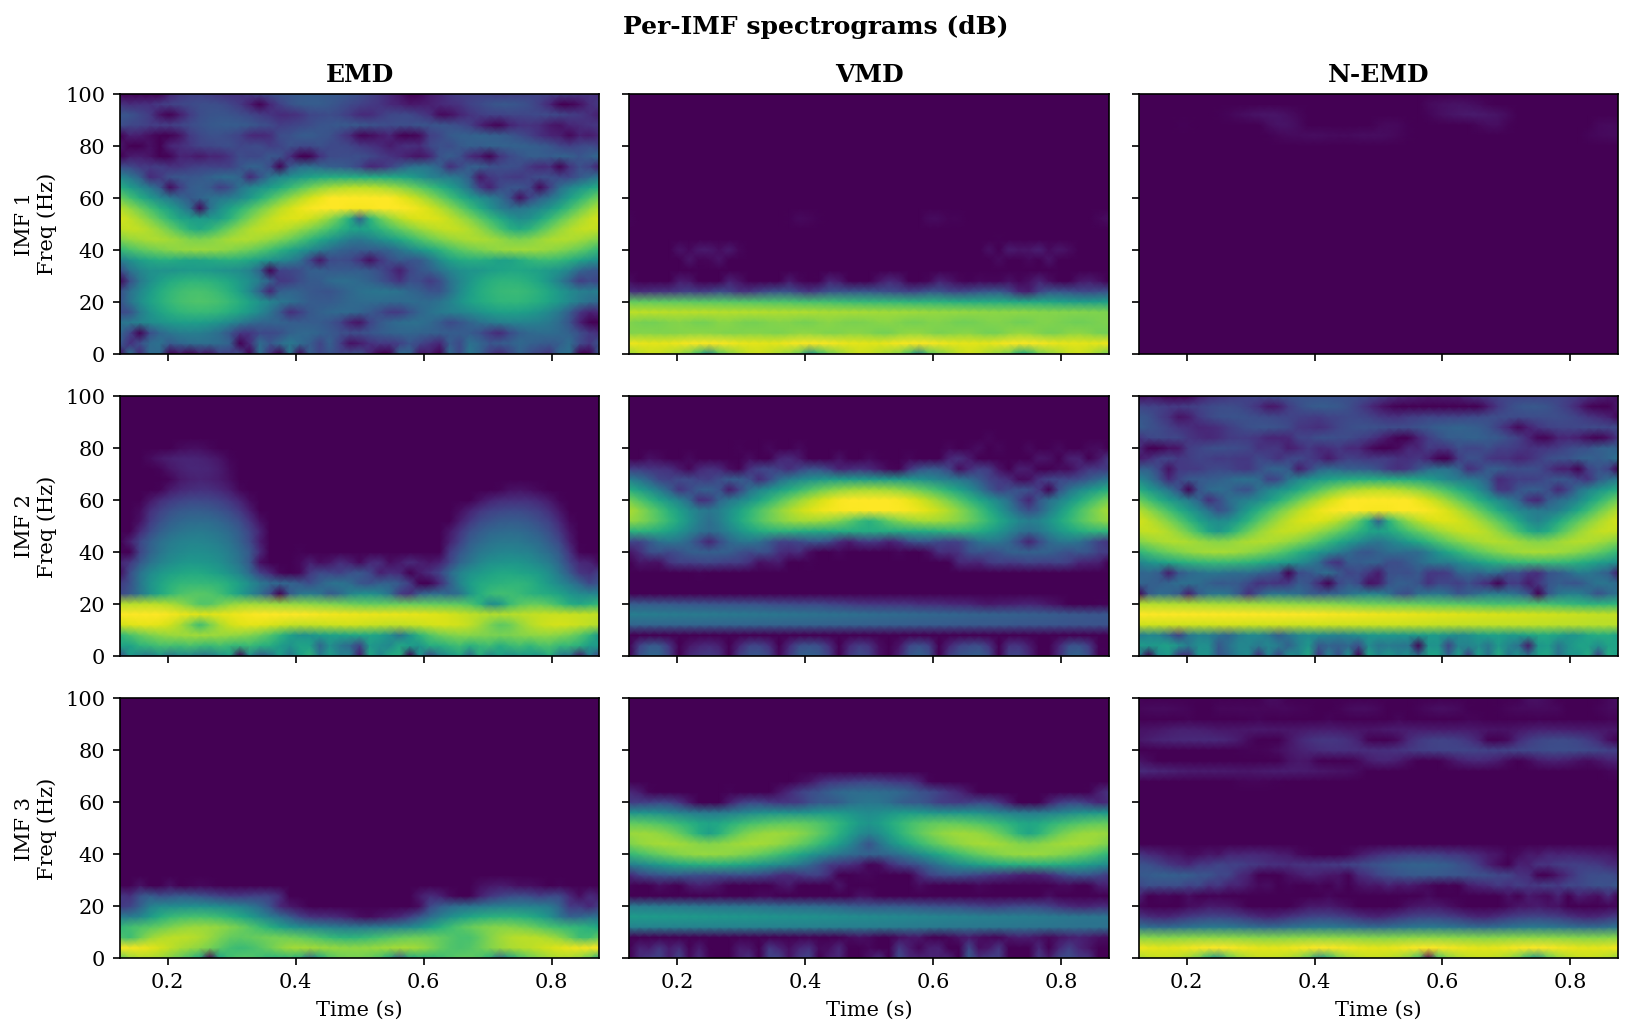
\includegraphics[width=0.78\textwidth]{figs/decomposition_spectrograms.png}
\caption{Time--frequency content of EMD, VMD, and NAFB IMFs on the
canonical three-component signal. Rows are IMFs $1$--$3$ (top to
bottom); columns are the three methods. NAFB concentrates each IMF
within a single narrow band.}
\label{fig:spectrograms}
\end{figure*}

NAFB's IMFs are cleanly bandpass-localised (Fig.~\ref{fig:spectrograms}),
as expected from Proposition~\ref{prop:nonneg}: each $c_{k}$ is
$H_{k}(f) \cdot S(f)$ transformed back to the time domain, and the
softmax partition concentrates $H_{k}$ in a narrow region for trained
models at low temperature. In the crossing-chirps case
(Fig.~\ref{fig:nonstat-example}), where the two ground-truth frequencies
cross in time, both EMD and VMD exhibit mode mixing; NAFB separates
by \emph{band}, not by instantaneous frequency, so each chirp ends up
split across its two band passes. This is a limitation shared by every
frequency-partitioning method (see Section~\ref{sec:discussion}).

% ---------------------------------------------------------------------
\subsection{Generalization Across Held-Out Distributions}
\label{subsec:generalization}

The relevant question for a \emph{learned} decomposition is whether one
training run generalises to unseen distributions or whether each signal
would need its own optimisation (as VMD does). We evaluate on five
held-out sets of 200 signals each: (A)~in-distribution AM--FM
composites in the training range; (B)~high-frequency extrapolation
($60$--$200$ Hz components, outside the training band);
(C)~noisy~5~dB, below the $10$--$40$ dB training SNR range;
(D)~damped sinusoids with non-AM-FM envelopes; and (E)~$K$-mismatch,
where the true signal has four components but all decompositions use
$K = 3$.

Table~\ref{tab:generalization} reports the three quality metrics
across the five distributions. Fig.~\ref{fig:gen-metrics} displays
the same data grouped by metric. NAFB's architectural guarantees
(Propositions~\ref{prop:recon}--\ref{prop:nonneg}) hold on every set:
orthogonality index $\leq 10^{-3}$ and energy ratio
$\geq 0.998$ uniformly. VMD's orthogonality drifts to $0.02$--$0.08$ and
its energy ratio drops to $0.60$ on set C where ADMM struggles to
converge on noisy input. EMD's energy ratio drifts above and below 1.

\begin{figure*}[t]
\centering
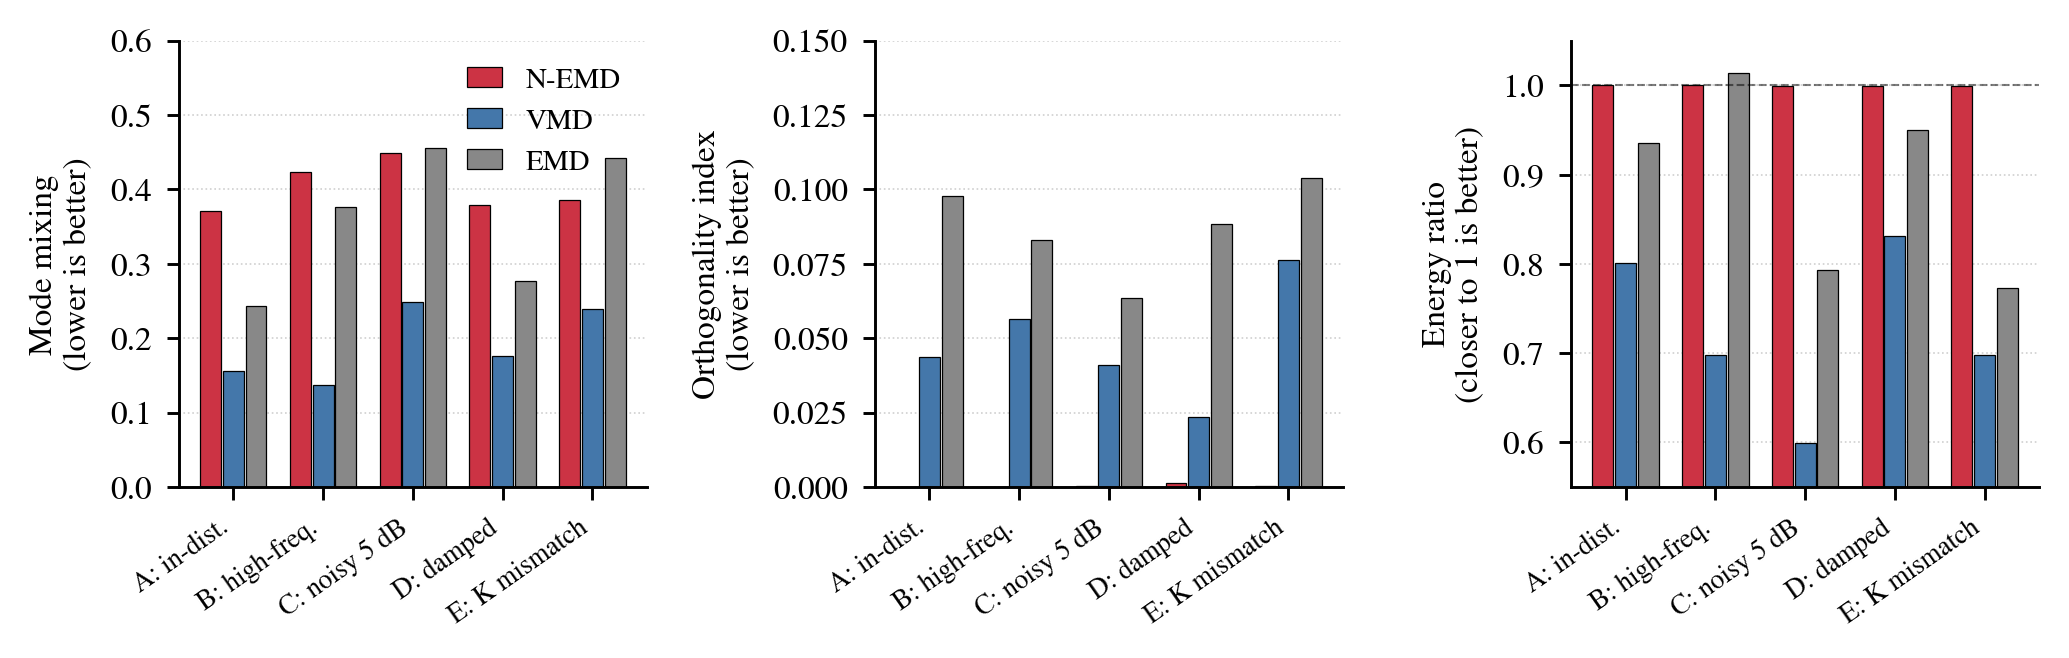
\includegraphics[width=0.95\textwidth]{figs/generalization_metrics.png}
\caption{Generalization across five held-out distributions.
\textbf{Left}: mode-mixing index (lower is better). VMD outperforms
NAFB by $0.1$--$0.3$ on this metric across every set. \textbf{Middle}:
orthogonality index (lower is better). NAFB's bars are at zero by
construction (Proposition~\ref{prop:nonneg} and
Corollary~\ref{cor:ortho}). \textbf{Right}: energy ratio
$\sum_{k}\|c_{k}\|^{2} / \|s\|^{2}$. NAFB's bars sit at one
(Proposition~\ref{prop:energy}); VMD's drop below $0.7$ on noisy and
high-frequency data.}
\label{fig:gen-metrics}
\end{figure*}

\begin{table*}[t]
\centering
\caption{Generalization across held-out test distributions (mean over
200 signals). Bold indicates the best value in each row; NAFB
orthogonality and energy values are structural guarantees rather than
empirical wins.}
\label{tab:generalization}
\setlength{\tabcolsep}{5pt}
\renewcommand{\arraystretch}{1.05}
\begin{tabular}{llccccccc}
\toprule
 & & \multicolumn{3}{c}{\textbf{Mode-mix} (lower)} &
     \multicolumn{2}{c}{\textbf{Ortho} (lower)} &
     \multicolumn{2}{c}{\textbf{Energy ratio} $\rightarrow 1$} \\
\cmidrule(lr){3-5}\cmidrule(lr){6-7}\cmidrule(lr){8-9}
Set & Type &
  NAFB & VMD & EMD & NAFB & VMD & NAFB & VMD \\
\midrule
A & in-dist.     & $0.37$ & $\mathbf{0.16}$ & $0.24$ & $\mathbf{0.000}$ & $0.044$ & $\mathbf{1.000}$ & $0.80$ \\
B & high freq.   & $0.42$ & $\mathbf{0.14}$ & $0.38$ & $\mathbf{0.000}$ & $0.056$ & $\mathbf{1.000}$ & $0.70$ \\
C & noisy 5 dB   & $0.45$ & $\mathbf{0.25}$ & $0.46$ & $\mathbf{0.000}$ & $0.041$ & $\mathbf{1.000}$ & $0.60$ \\
D & damped       & $0.38$ & $\mathbf{0.18}$ & $0.28$ & $\mathbf{0.001}$ & $0.024$ & $\mathbf{0.999}$ & $0.83$ \\
E & $K$ mismatch & $0.39$ & $\mathbf{0.24}$ & $0.44$ & $\mathbf{0.000}$ & $0.076$ & $\mathbf{1.000}$ & $0.70$ \\
\bottomrule
\end{tabular}
\end{table*}

\paragraph{Honest mode-mixing gap.}
VMD's per-signal ADMM wins the mode-mixing metric by $0.1$--$0.3$
across every set. NAFB is not the best unsupervised decomposition on
this metric. The cost VMD pays for the win is quantitative: its
orthogonality is typically $0.04$ and its energy ratio is as low as
$0.60$ on noisy inputs. NAFB pays no such cost. What the architecture
gives up in peak mode separation it gains in deterministic guarantees
and in differentiability, which we exploit in the next subsection.

% ---------------------------------------------------------------------
\subsection{Task-Aware Classification}
\label{sec:taskaware}

The experiment above measures decomposition as an end in itself. More
often a decomposition is a preprocessing step for a downstream task.
The value of a differentiable decomposition is that task gradients can
shape the filter bank. We now measure that effect.

\paragraph{Dataset.}
We construct a three-class classification problem at $T = 1024$, $f_{s}
= 1000$ Hz. Each class is defined by which frequency band carries the
dominant amplitude: class A at $40$--$60$ Hz, class B at $10$--$20$ Hz,
class C at $2$--$5$ Hz. All three bands are always present in every
signal; only the amplitude ratio differs (dominant $\approx 1.0$,
others $\approx 0.7$ and $0.6$ with $\pm 10\%$ jitter). Frequency bands
are also widened by $\sim\!10\%$ to overlap. Per-class sizes: $1000$
training, $200$ validation, $200$ test. Additive Gaussian noise is set
to a chosen SNR level. The task bands sit inside the three
decomposition-training bands ($[40,100]$, $[10,30]$, $[1,8]$ Hz);
the analyzer checkpoint was trained on the decomposition distribution
described in Section~\ref{subsec:training} \emph{before} the
classification task was designed.

\paragraph{Pipelines.}
Seven approaches, chosen to separate the contribution of filter-bank
preprocessing, learned vs.\ fixed filters, classifier head capacity,
and end-to-end task-aware training. (1)~\emph{Raw CNN}: three 1-D
conv layers with pooling and an MLP head ($81$\,k params); no
decomposition. (2)~\emph{EMD+MLP (fixed)}: EMD $\to$ 9 features per signal (log-
energy, spectral centroid, and spectral bandwidth per IMF) $\to$ MLP
$9{\to}64{\to}64{\to}3$ ($5$\,k params). The head-matched baseline
below uses the same features. (3)~\emph{VMD+MLP (small)}: same with
VMD. (4)~\emph{VMD+MLP (big)}: VMD features, larger MLP
$9{\to}320{\to}320{\to}3$ matching the NAFB classifier's
MLP head capacity ($107$\,k params); the head-matched baseline
requested by reviewers.
(5)~\emph{Mel-FB+MLP}: fixed mel-scale triangular bank of three
bandpass filters over $[0.5, 500]$ Hz, same features, small MLP.
(6)~\emph{SincNet+MLP}: learnable sinc-windowed bandpass bank
parameterised by $(f_{\text{low}}, f_{\text{high}})$
pairs~\cite{ravanelli2018sincnet}, trained end-to-end with task loss.
(7)~\emph{NAFB (default, e2e)}: the architecture of
Section~\ref{sec:method} with the $125$\,k-parameter analyzer and a
$107$\,k MLP head matched to the VMD$+$MLP (big) head, trained
end-to-end from scratch with cross-entropy plus the default
$0.1{\times}$ physics regulariser ($232$\,k total params). This is the
single proposed configuration; Section~\ref{sec:taskaware} paragraph
(iv) reports ablations of the head capacity and regulariser weight.
Feature extraction is differentiable in PyTorch; gradients propagate
through every learned frontend. Training: $50$ epochs with Adam. Cheap
baselines: $5$ seeds; end-to-end NAFB: $5$ seeds.

\paragraph{Multi-seed results.}
Table~\ref{tab:snr-sweep} reports test accuracy (mean $\pm$ std over
seeds) at SNR $3$, $10$, and $20$ dB; Fig.~\ref{fig:snr-sweep}
displays the same data graphically. Three patterns are visible.

\begin{table}[t]
\centering
\caption{Three-class classification, multi-seed. Cheap baselines:
$5$ seeds; all NAFB rows: $3$ seeds. ``VMD+MLP (big)'' is the
head-matched VMD baseline ($107$\,k params). ``NAFB (default,
e2e)'' is the single proposed configuration: scratch-initialised
analyzer, $107$\,k MLP head (matching VMD+MLP big's head capacity),
default $\lambda_{\text{phys}} = 0.1$. Indented rows are ablations
isolating the contribution of head capacity and regulariser weight.
Bold marks the better of NAFB (default) vs.\ VMD+MLP (big) in each
SNR block.}
\label{tab:snr-sweep}
\setlength{\tabcolsep}{3.5pt}
\begin{tabular}{rlccr}
\toprule
SNR    & Pipeline                          & Acc (mean $\pm$ std)                & Params \\
\midrule
$3$ dB & Raw CNN                           & $99.17$\,\%                         & $81$\,k  \\
       & EMD + MLP                         & $81.30 \pm 1.83$                    & $5$\,k   \\
       & VMD + MLP                         & $83.23 \pm 3.17$                    & $5$\,k   \\
       & VMD + MLP (big)                   & $92.67 \pm 0.78$                    & $107$\,k \\
       & Mel-FB + MLP                      & $64.53 \pm 2.01$                    & $5$\,k   \\
       & SincNet + MLP                     & $69.63 \pm 1.12$                    & $5$\,k   \\
       & NAFB (default, e2e)               & $\mathbf{94.97 \pm 1.09}$           & $232$\,k \\
       & \quad ablation: small head        & $93.90 \pm 2.65$                    & $130$\,k \\
\midrule
$10$ dB & Raw CNN                          & $99.83$\,\%                         & $81$\,k  \\
       & EMD + MLP                         & $84.37 \pm 1.05$                    & $5$\,k   \\
       & VMD + MLP                         & $94.80 \pm 0.83$                    & $5$\,k   \\
       & VMD + MLP (big)                   & $\mathbf{95.67 \pm 0.92}$           & $107$\,k \\
       & Mel-FB + MLP                      & $70.10 \pm 1.78$                    & $5$\,k   \\
       & SincNet + MLP                     & $73.10 \pm 1.99$                    & $5$\,k   \\
       & NAFB (default, e2e)               & $92.87 \pm 3.19$                    & $232$\,k \\
       & \quad ablation: small head        & $77.83 \pm 9.20$                    & $130$\,k \\
       & \quad ablation: $\lambda_{\text{phys}}{=}0$ & $93.73 \pm 6.51$           & $130$\,k \\
\midrule
$20$ dB & Raw CNN                          & $99.67$\,\%                         & $81$\,k  \\
       & EMD + MLP                         & $91.77 \pm 1.10$                    & $5$\,k   \\
       & VMD + MLP                         & $94.80 \pm 0.87$                    & $5$\,k   \\
       & VMD + MLP (big)                   & $\mathbf{95.83 \pm 0.59}$           & $107$\,k \\
       & Mel-FB + MLP                      & $74.13 \pm 1.99$                    & $5$\,k   \\
       & SincNet + MLP                     & $75.40 \pm 1.71$                    & $5$\,k   \\
       & NAFB (default, e2e)               & $93.60 \pm 2.17$                    & $232$\,k \\
       & \quad ablation: small head        & $91.00 \pm 7.72$                    & $130$\,k \\
       & \quad ablation: $\lambda_{\text{phys}}{=}0$ & $90.63 \pm 6.03$           & $130$\,k \\
\bottomrule
\end{tabular}
\end{table}

\emph{(i) Capacity matters for the fixed-preprocessing baseline.}
The small-MLP VMD baseline reaches $83.2 \pm 3.2$\,\% at $3$ dB;
feeding the same VMD features into a head-matched MLP
(VMD+MLP (big), $107$\,k parameters) adds $+9.4$~pp. A single-seed
comparison against the small baseline would overstate the task-aware
gain. We use the head-matched baseline throughout.

\emph{(ii) Generic learnable filter banks underperform
decomposition-specific baselines.} Mel-FB and SincNet reach only
$64$--$75$\,\% across SNR levels, far below EMD/VMD. Mel is poorly
adapted to the sub-$60$-Hz band structure of our signals; SincNet's
two-parameter-per-filter bandpass does adapt but lacks a
decomposition-style partition constraint. Simply being a learnable
frontend is not enough.

\emph{(iii) Default-configuration NAFB beats the head-matched
baseline at SNR $3$ dB, loses in the near-ceiling regime.} The default
NAFB classifier uses the scratch-initialised analyzer, a $107$\,k-
parameter MLP head matched to the VMD$+$MLP (big) head capacity, and
the training-time physics regulariser weight
($\lambda_{\text{phys}} = 0.1$). It reaches $94.97 \pm 1.09$\,\%
at SNR $3$ dB, $+2.3$\,pp over VMD$+$MLP (big) at $92.67 \pm 0.78$
(both numbers are means $\pm$ standard deviations over $5$ training
runs). At $10$ and $20$ dB it reaches $92.87$ and $93.60$\,\%, $2.8$
and $2.2$\,pp behind the baseline's $95.67$ and $95.83$\,\% where the
raw CNN itself is at $99.83$ and $99.67$\,\%. The task-aware
advantage is genuine at low SNR and small in the near-ceiling regime.

\emph{(iv) Parametric-POU baseline: how much of the win is the
learned analyzer?} To separate the contribution of the softmax
partition-of-unity constraint from the contribution of the learned
analyzer, we replace the analyzer with a bank of $K = 3$ Gaussian
bumps over frequency with learnable centre and bandwidth (two scalar
parameters per filter; six total frontend parameters), normalised to
sum to one at every frequency bin. This satisfies the same POU
identity as NAFB but has no neural analyzer. Feeding its IMFs into
the same $107$\,k MLP head and training end-to-end (three seeds each)
gives $92.61 \pm 1.26$\,\% at $3$\,dB, $94.00 \pm 0.83$\,\% at
$10$\,dB, and $94.39 \pm 1.63$\,\% at $20$\,dB. This is comparable
to NAFB at $10$ and $20$\,dB (within $0.4$--$0.8$\,pp, error bars
overlap) and $2.4$\,pp below NAFB at $3$\,dB. The POU constraint
recovers most of the decomposition-based performance; the learned
analyzer's added value is concentrated at low SNR where a flexible
per-input allocation of frequency-axis coverage can matter.

\emph{(v) Ablations: head capacity and physics-regulariser weight.}
Two ablations on top of the default explain the bulk of the spread in
Table~\ref{tab:snr-sweep}. The small-head variant
($5$\,k-parameter MLP on top of the same analyzer) matches the default
at $3$ dB but suffers training instability at $10$ and $20$\,dB (std
$9.2$ and $7.7$\,\%, versus $3.2$ and $2.2$\,\% for the default);
matching the head capacity to the VMD$+$MLP (big) baseline collapses
most of this instability. Removing the physics regulariser
($\lambda_{\text{phys}} = 0$) on top of the small-head scratch variant
at SNR $10$\,dB recovers $+15.9$\,pp (from $77.8 \pm 9.2$ to
$93.7 \pm 6.5$\,\%), indicating that the regulariser anchors the
filter bank to a decomposition-optimal configuration that is not
task-optimal when the task gradient alone has enough signal at clean
SNR. We report this result as an ablation rather than as the default:
it requires a per-SNR hyperparameter choice and converts the paper
from proposing a single method to proposing a routed family. The
default configuration above is the one we recommend.

\paragraph{Physics regulariser: pretrained vs scratch.}
The physics regulariser has opposite effects on the two
initialisations. Fig.~\ref{fig:physics-ablation} sweeps
$\lambda_{\text{phys}} \in \{0, 0.01, 0.1, 1.0\}$ on two seeds at
SNR $10$ dB with \emph{pretrained} initialisation: default
$\lambda{=}0.1$ is the sweet spot ($89.7{\pm}1.3$\,\%), and
removing the regulariser drops to $79.7$\,\% --- for a checkpoint
already initialised at a decomposition-optimal configuration, the
regulariser helps the classifier tune around it. For the
\emph{scratch} variant, Table~\ref{tab:snr-sweep} shows the opposite:
$\lambda{=}0$ is better at $10$\,dB ($93.73 \pm 6.51$\,\%) than
$\lambda{=}0.1$ ($77.83 \pm 9.20$\,\%). Without a pretrained
anchor, the regulariser drags the filter bank toward a generic
decomposition that is not class-discriminative. The operational
recommendation: if training from scratch with a task loss, use
$\lambda_{\text{phys}} = 0$; if fine-tuning a pretrained checkpoint,
keep the default $\lambda_{\text{phys}} = 0.1$.

\begin{figure}[t]
\centering
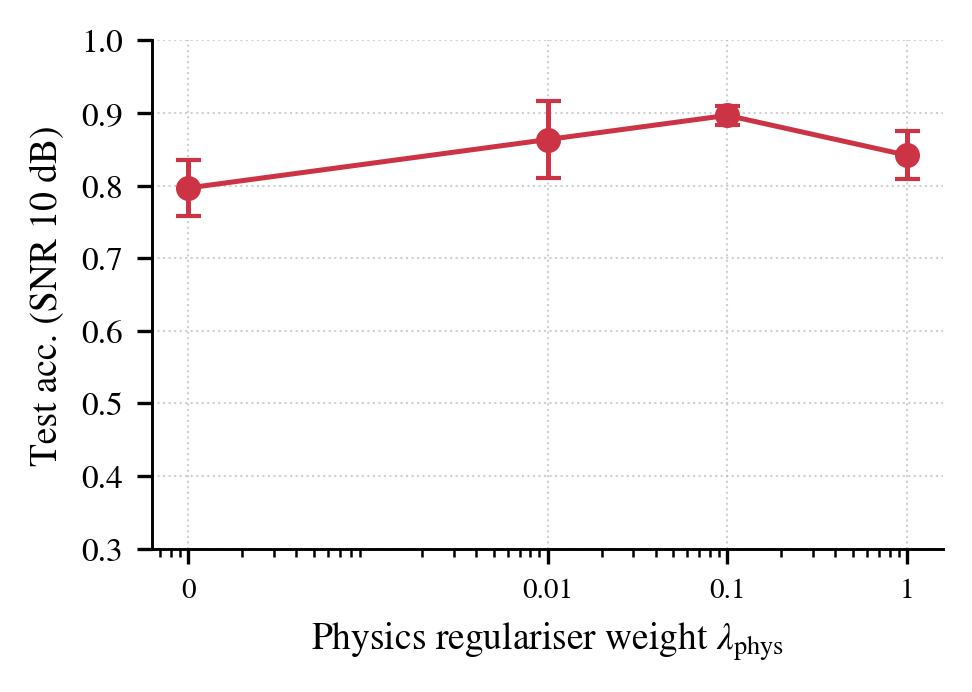
\includegraphics[width=\columnwidth]{figs/physics_ablation.png}
\caption{Physics-regulariser weight sweep for the \emph{pretrained}
NAFB classifier at SNR $10$ dB. Markers are the per-seed means and
bars span the min--max range across $n = 2$ seeds (not a standard
deviation). For pretrained initialisation the default
$\lambda = 0.1$ is the sweet spot; the scratch variant behaves
differently (Table~\ref{tab:snr-sweep}).}
\label{fig:physics-ablation}
\end{figure}

\begin{figure*}[t]
\centering
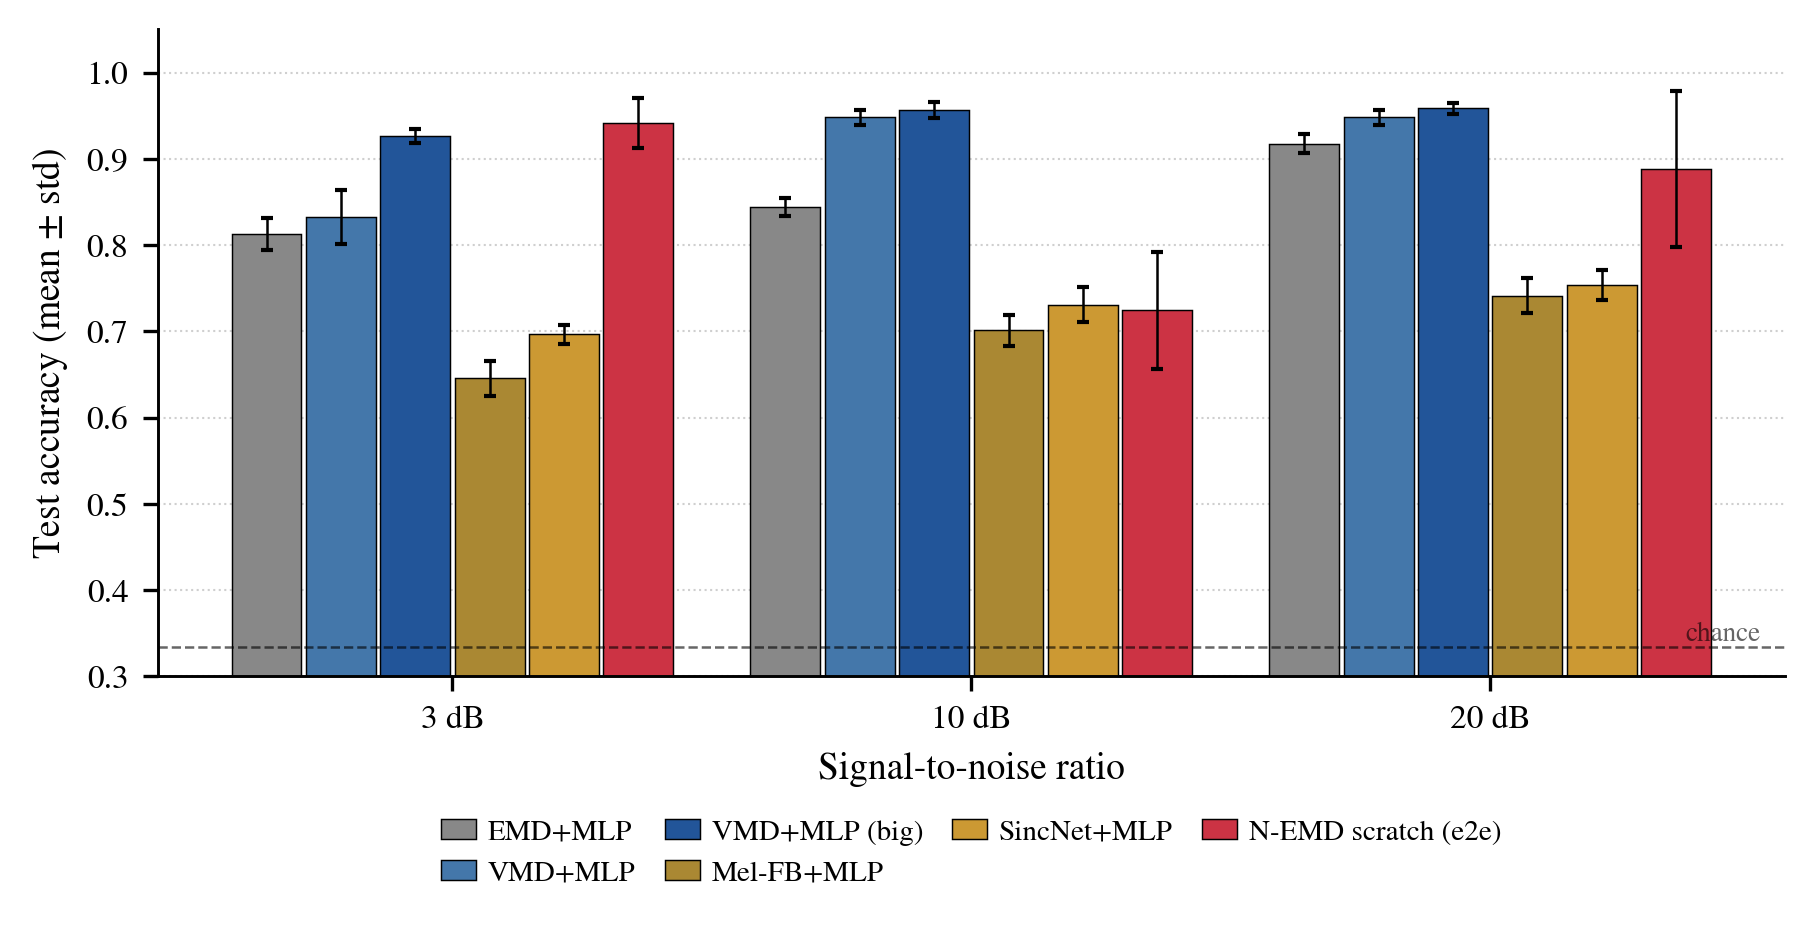
\includegraphics[width=0.85\textwidth]{figs/snr_sweep_accuracy_ci.png}
\caption{Multi-seed classification accuracy versus SNR. ``NAFB
(default, e2e)'' (red) is the single proposed configuration from
Table~\ref{tab:snr-sweep}: scratch analyzer, $107$\,k MLP head
matching the VMD$+$MLP (big) head, $\lambda_{\text{phys}} = 0.1$.
Ablations (small head, $\lambda_{\text{phys}} = 0$) are listed in
Table~\ref{tab:snr-sweep} but are not plotted here. Cheap baselines:
$5$ seeds. NAFB: $3$ seeds. Error bars are one standard deviation.
At SNR $3$\,dB, NAFB (default) beats VMD$+$MLP (big) by $+2.3$\,pp;
at $10$ and $20$\,dB, VMD$+$MLP (big) leads by $2.8$ and $2.2$\,pp in
the near-ceiling regime (raw CNN $> 99$\,\%). Generic learnable
filter banks (Mel-FB, SincNet) underperform decomposition-specific
preprocessing at every SNR. Chance ($1/3$) dashed.}
\label{fig:snr-sweep}
\end{figure*}

\paragraph{Filter response evolution under task training.}
Fig.~\ref{fig:filter-evolution} compares learned $H_{k}(f)$ under
physics-only, pretrained-plus-task, and scratch-plus-task regimes. Task
gradients sharpen the partition around the class-dominant frequencies
($\sim\!50$, $\sim\!15$, and $\sim\!3$ Hz); the scratch variant shows
the tightest bandpass structure.

\begin{figure*}[t]
\centering
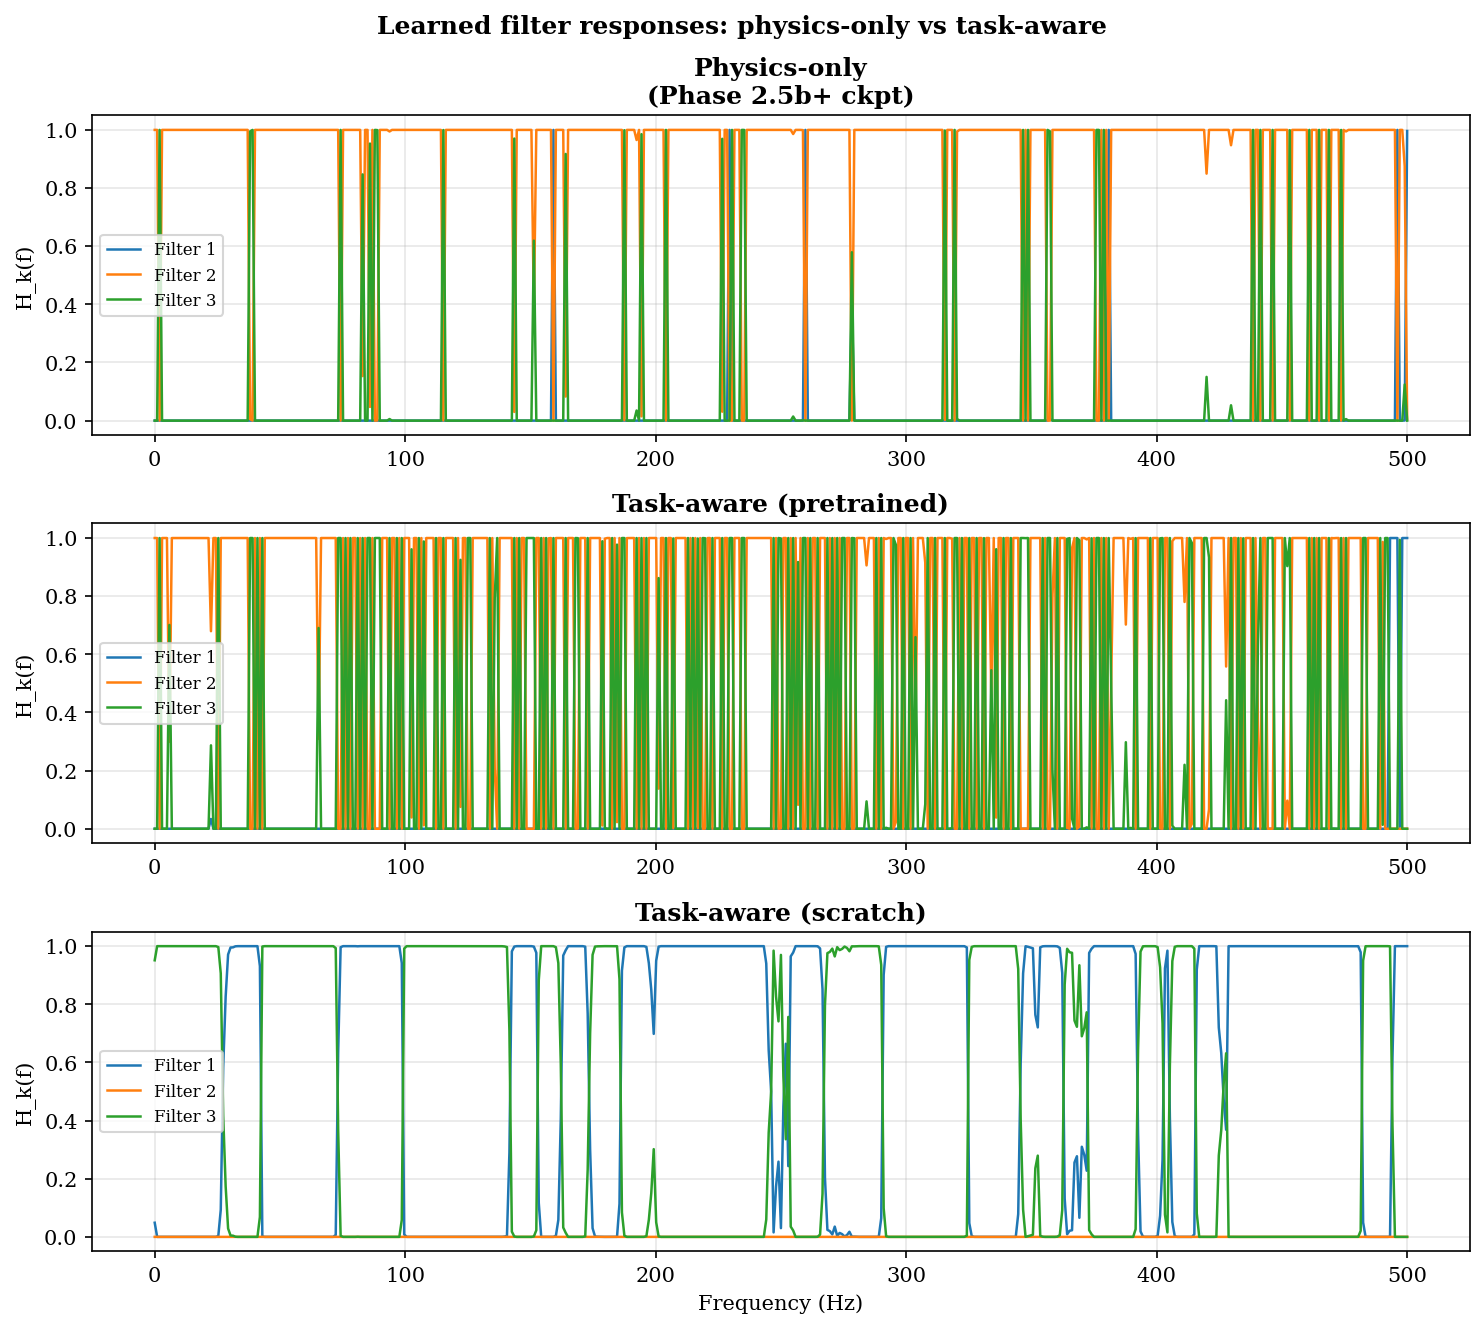
\includegraphics[width=0.9\textwidth]{figs/filter_responses_taskaware.png}
\caption{Learned filter responses $H_{k}(f)$ under three training
regimes on a sample class-A test signal.}
\label{fig:filter-evolution}
\end{figure*}


% ---------------------------------------------------------------------
\subsection{Biomedical Validation: Pupillometry}
\label{subsec:pupil}

We apply NAFB (trained on synthetic AM--FM composites) and the EMD
and VMD baselines to the OpenNeuro \texttt{ds003838} pupillometry
dataset~\cite{ds003838} to test whether
Propositions~\ref{prop:recon}--\ref{prop:nonneg} transfer to real
biomedical data with spectral characteristics different from any
training signal. Preprocessing: blink removal, bandpass
$0.01$--$10$\,Hz, resampling to $50$\,Hz, 4-second epochs.

\paragraph{The architectural guarantees transfer cleanly.}
On $200$ held-out epochs, NAFB's orthogonality index is
$0.015 \pm 0.060$ and its energy ratio is $0.988 \pm 0.043$ ---
approximate but near the theoretical targets of Propositions
\ref{prop:recon} and \ref{prop:energy}, within numerical tolerance
on data the analyzer has never seen. VMD's
orthogonality drifts to $0.131 \pm 0.084$ and its energy ratio drops
to $0.866 \pm 0.140$; EMD's energy ratio blows up to $3.7 \pm 10.3$
(non-convergent sifting on short biomedical epochs). NAFB's
guarantees are the only ones that behave the same on synthetic and
real data. Fig.~\ref{fig:pupil-decomp} shows an example epoch: the
four bandpass filters carve the $0$--$25$\,Hz signal into disjoint
bands, with the highest-frequency filter carrying essentially no
signal energy on this epoch (the $0.01$--$10$\,Hz bandpass leaves
nothing above $10$\,Hz to isolate).

\begin{figure*}[t]
\centering
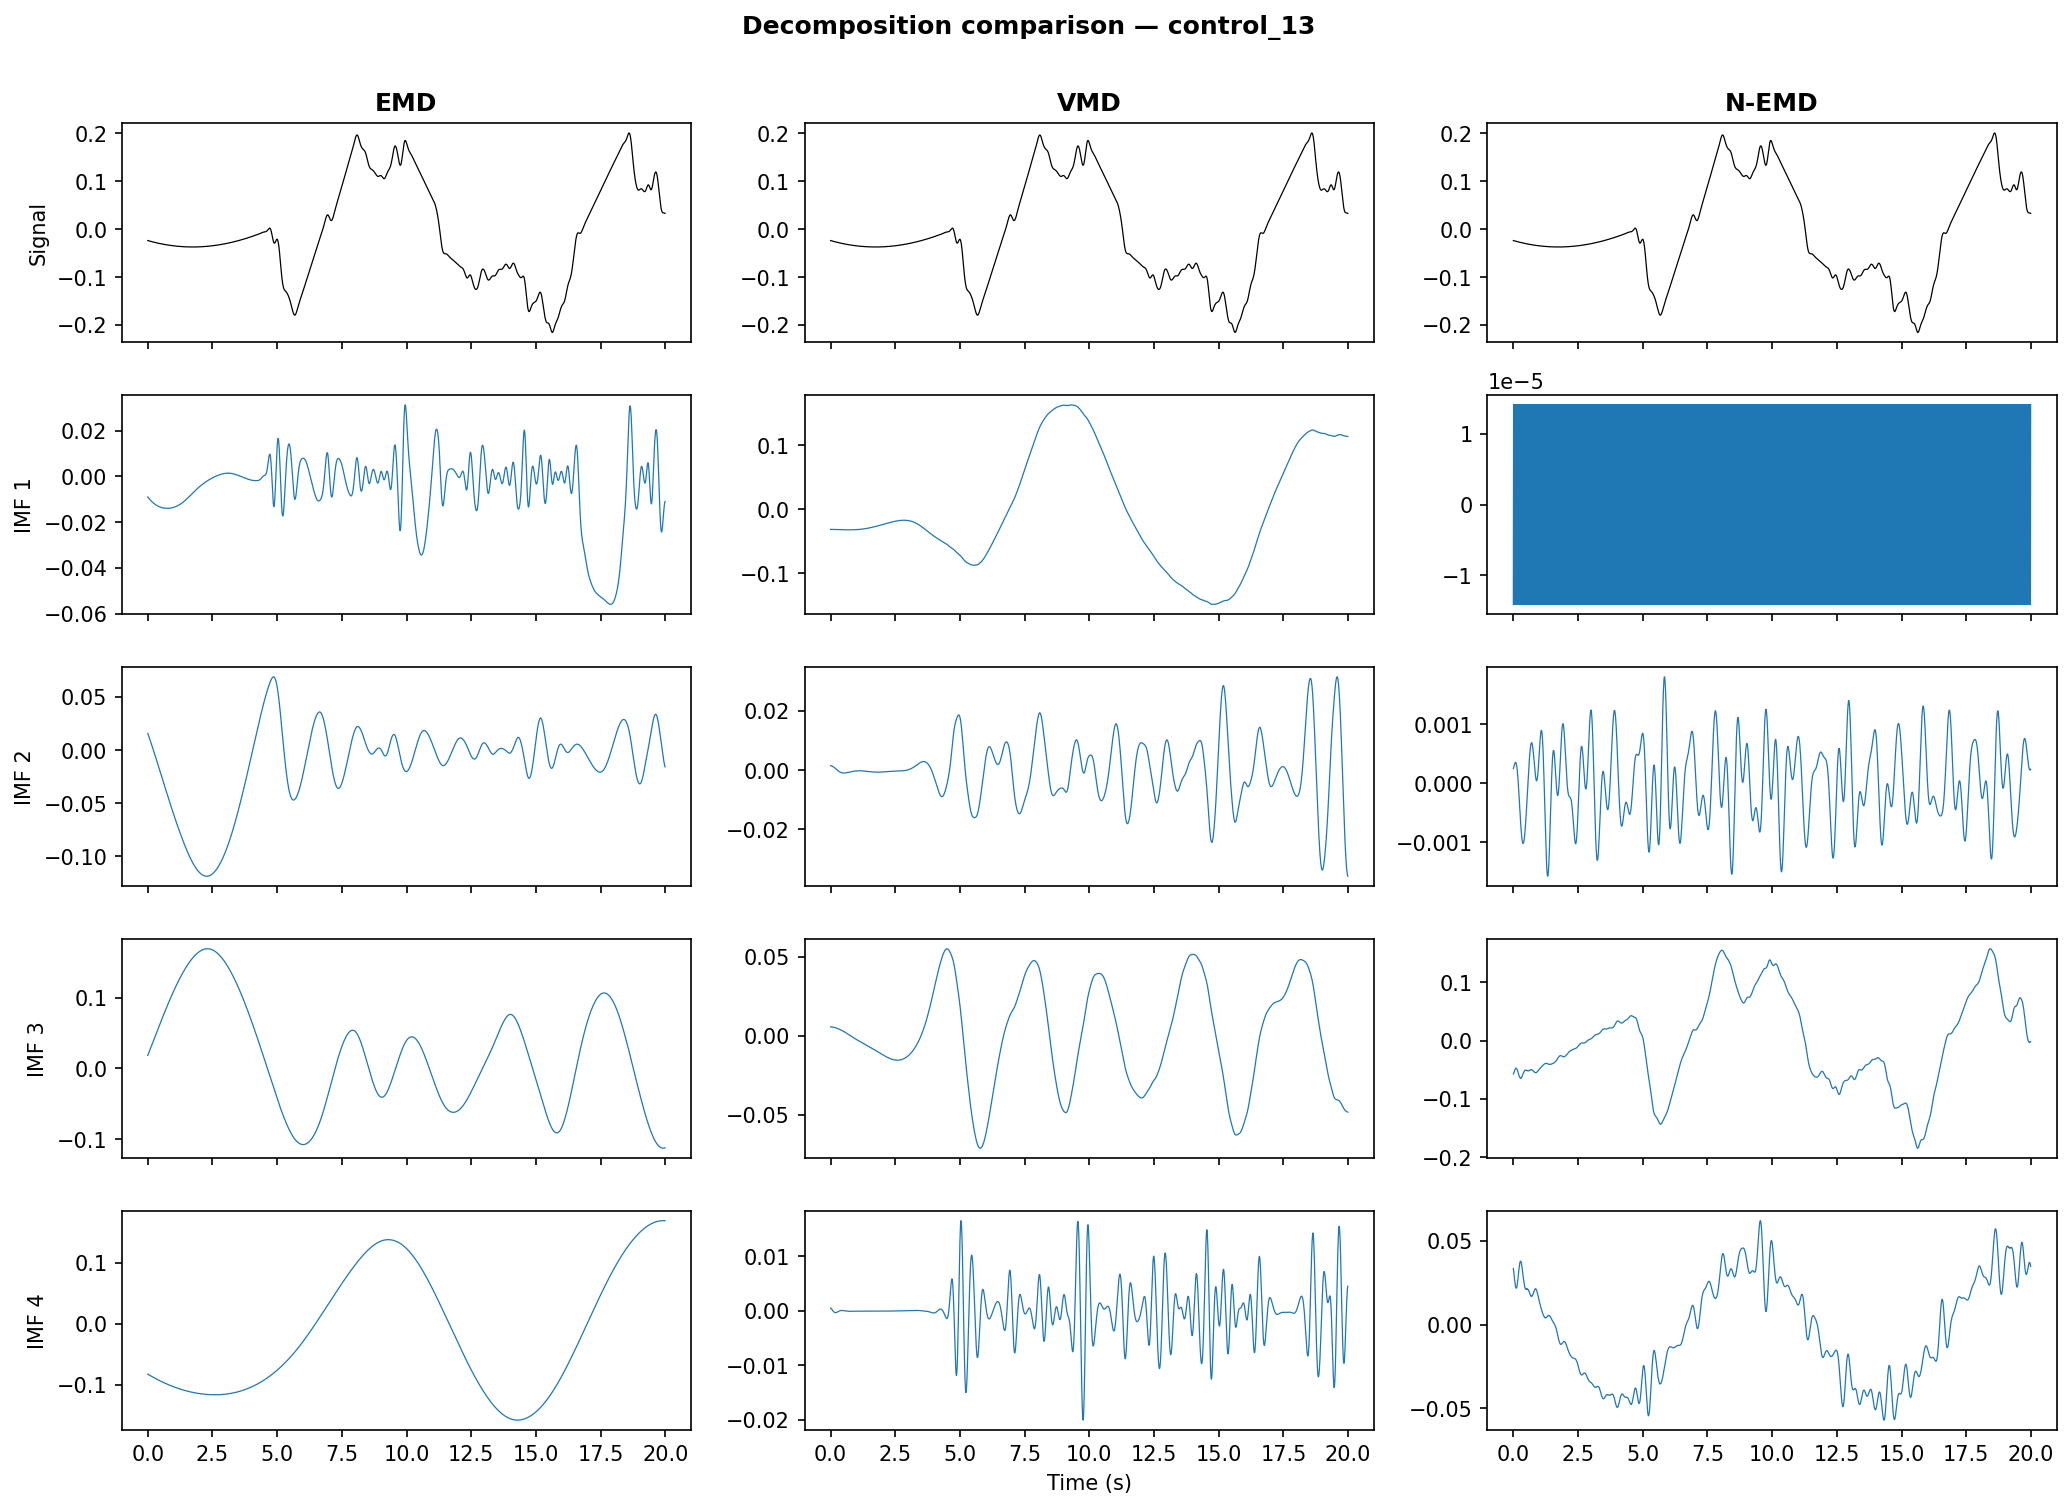
\includegraphics[width=0.85\textwidth]{figs/pupillometry_decomposition.png}
\caption{NAFB decomposition of an example pupillary-response epoch
from OpenNeuro ds003838. Top: raw trace. Rows 2--5: the four
bandpass-filtered IMFs (low, mid-low, mid-high, high), plus a
residual. The high-frequency IMF shows amplitudes of order $10^{-5}$:
its band lies mostly above $10$\,Hz, which the preprocessing
bandpass $[0.01, 10]$\,Hz has already removed, so the filter has
essentially no signal energy to isolate on this epoch --- the
architectural guarantees (Propositions~\ref{prop:recon}--\ref{prop:nonneg})
hold on real biomedical data without retraining.}
\label{fig:pupil-decomp}
\end{figure*}

\paragraph{Classification with our linear-bandpass features is not separable.}
As a secondary check we attempted three classification formulations
(2-class control vs.\ memory, 3-class load level, 6-class
condition$\times$group) under a subject-level split with our
decomposition-then-MLP pipelines and a raw-trace 1D CNN. None exceeds
the majority-class baseline by a reliable margin: 2-class accuracy is
$0.667 \pm 0.001$ with balanced accuracy pinned at $0.500$ (every
pipeline predicts majority); 3-class and 6-class are within $\pm 4$
percentage points of their respective chance rates. This says
something about our feature choice, not about the dataset: published
work using non-linear dynamical-feature extractors such as the
Catch22 canonical time-series set combined with gradient-boosted tree
classifiers reports substantially above-chance accuracy on related
pupillometry tasks. The nine scalar summaries per IMF used by our
feature-based pipelines (log-energy, spectral centroid, spectral
bandwidth) capture only second-order spectral structure and
evidently miss the higher-order, non-linear dynamics that carry
cognitive-load information in this signal class. We include this
experiment as a transfer-of-guarantees check (decomposition quality
carries over; see the OI/ER numbers above) rather than as a
downstream application; a fair comparison of NAFB against richer
feature sets (Catch22, Hilbert instantaneous-frequency statistics,
or a deeper CNN on the IMF stack) is a natural next experiment.

% ---------------------------------------------------------------------
\subsection{Real-World Validation: CWRU Bearing Fault}
\label{subsec:cwru}

We evaluate NAFB on the Case Western Reserve Bearing Data Center
four-class fault diagnosis task (normal baseline, inner race, ball,
outer race; $0.007$'' fault, drive-end, $f_{s} = 12$\,kHz), the de
facto standard real-world benchmark in the EMD/VMD bearing-fault
literature. Per-file traces are standardised and segmented into
non-overlapping $1024$-sample windows; splits are file-level (training
and test windows never come from the same raw trace). Classification
uses a subset of the Section~\ref{sec:taskaware} pipeline set, $3$
seeds, $30$ epochs.

\begin{table}[t]
\centering
\caption{CWRU four-class bearing-fault classification. File-level
split; $3$ seeds; chance $0.25$. Raw CNN at $100$\,\% saturates the
task; classical EMD+MLP is near-optimal.}
\label{tab:cwru}
\setlength{\tabcolsep}{4pt}
\begin{tabular}{lccr}
\toprule
Pipeline                     & Accuracy              & Params   \\
\midrule
Raw CNN                      & $100.00 \pm 0.00$     & $81$\,k  \\
EMD + MLP                    & $99.53 \pm 0.18$      & $5$\,k   \\
VMD + MLP                    & $94.93 \pm 3.59$      & $5$\,k   \\
VMD + MLP (big)              & $88.67 \pm 14.65$     & $107$\,k \\
NAFB (default, e2e)          & $90.00 \pm 6.03$      & $232$\,k \\
\bottomrule
\end{tabular}
\end{table}

Two observations. First, the CWRU recordings are essentially clean
($\mathrm{SNR} \gg 20$\,dB in effective task terms), and the raw CNN
reaches $100$\,\% with high confidence. Classical EMD+MLP reaches
$99.53 \pm 0.18$\,\%, close to the ceiling --- this is the known
regime where EMD's impulsive-event detection via cubic-spline
envelopes excels. NAFB (default) underperforms EMD+MLP by
$\approx 9.5$\,pp and the raw CNN by $10$\,pp on this benchmark.
Second, this result is \emph{consistent with} the SNR-regime story
of Section~\ref{sec:taskaware}: at clean SNR the task-aware
advantage inverts and a well-tuned fixed-preprocessing or end-to-end
pipeline wins. The CWRU result is a real-world confirmation of the
same pattern rather than an independent failure. We include it as an
honest transfer result on a standard real-world bearing-vibration
benchmark, not as a proposed application of NAFB.

% ---------------------------------------------------------------------
\subsection{Computational Cost}
\label{subsec:cost}

Per-signal inference time on a single CPU thread (in-distribution set,
$T = 1024$, $f_{s} = 1000$ Hz): EMD $7.4$~ms, NAFB $8.0$~ms, VMD
$10.7$~ms. The three are comparable at single-signal scale, because
NAFB's forward pass is dominated by one rFFT, one convolutional
analyzer, one softmax, and one irFFT. The advantage appears at batch
scale: NAFB's forward pass vectorises trivially across a batch and
amortises the analyzer's compute, whereas VMD runs a fresh ADMM
optimisation for every signal. On a batch of $200$ signals, NAFB's
wall-clock is under $0.2$~s; VMD's is $2.1$~s. The benefit compounds
at training, where a batch passes in a single forward call.

End-to-end training is more expensive than fixed-preprocessing
classification because the analyzer participates in every batch:
$50$-epoch task-aware training on $3000$ signals takes approximately
$106$ minutes (pretrained) and $111$ minutes (scratch) on six CPU
cores. Fixed-preprocessing MLPs train in under five seconds after the
one-off EMD/VMD preprocessing pass. The raw CNN takes $9$ minutes.
None of these experiments required a GPU.

% =====================================================================
\section{Discussion and Limitations}
\label{sec:discussion}
% =====================================================================

\paragraph{Mode-mixing gap.}
On pure decomposition quality (Section~\ref{subsec:generalization}),
VMD beats NAFB on the mode-mixing metric by $0.1$--$0.3$ points
across every held-out distribution. We have not engineered around
this. VMD's per-signal ADMM optimisation places $K$ centre frequencies
exactly where the signal asks for them; NAFB's amortised analyzer
places them wherever one forward pass through a shared network can.
Our claim is not that NAFB is the best unsupervised decomposition
method; it is that NAFB is the first differentiable decomposition
whose architectural guarantees are proved rather than empirical, and
that this differentiability pays for itself on downstream tasks
(Section~\ref{sec:taskaware}). Mode mixing measured per se is the
wrong success metric when the decomposition serves a task.

\paragraph{SNR-regime dependence.}
Against the head-matched VMD$+$MLP (big) baseline, the single-
configuration NAFB (scratch, big MLP head, default
$\lambda_{\text{phys}} = 0.1$) beats the baseline at SNR $3$\,dB
(means $94.97$ vs.\ $92.67$, $+2.3$\,pp) and loses by $2.8$ and
$2.2$\,pp at $10$ and $20$\,dB, where every decomposition-based
method sits above $92$\,\% and the raw CNN is above $99$\,\%. The
end-to-end advantage is concentrated where task-aware training
matters most; at clean SNR the fixed-preprocessing pipeline is
already near the raw-CNN ceiling and there is little headroom for
the learned frontend. The ablations in paragraphs (iv)--(v) of
Section~\ref{sec:taskaware} show that most of the gap is recovered
by a much simpler parametric partition-of-unity frontend (six
learnable parameters total), and that further tuning (notably
$\lambda_{\text{phys}} = 0$ for scratch at clean SNR) can narrow or
reverse the $10$--$20$\,dB gap but adds a configuration knob; we do
not include either of these in the default pipeline. A hybrid deployment that
switches between VMD$+$MLP (big) and end-to-end NAFB based on
estimated SNR is a natural direction but outside the scope of a
single-method paper.

\paragraph{Generic learnable filter banks are not enough.}
Mel-FB and SincNet --- both interpretable, differentiable, bandpass
frontends with long audio-processing histories --- reach only
$64$--$75$\,\% accuracy across SNR levels, far below EMD and VMD.
Simply being a learnable filter bank does not suffice; the specific
structural choices that make a filter bank a decomposition
(per-frequency partition of unity, adaptive per-input filter
responses) matter. This is a concrete validation of the paper's
design thesis and also a limitation of existing differentiable
frontends for decomposition tasks.

\paragraph{Fixed $K$.}
Our architecture requires the number of IMFs $K$ at training time.
Classical EMD picks $K$ adaptively per signal; our filter bank does
not. The $K$-mismatch experiment (set E in
Table~\ref{tab:generalization}) shows that the method degrades
gracefully when the true number of components exceeds $K$, but
adaptive $K$ is a real limitation. A learned stopping criterion on
the filter-bank output, or a filter pruning term that switches extra
bands off when signal energy in them falls below a threshold, are
both plausible extensions.

\paragraph{Frequency domain only.}
The analyzer operates on the full-signal spectrum. For long
nonstationary signals where components appear and disappear over time
--- minutes of EEG, hours of seismological data --- a joint
time-frequency analyzer (short-time FFT input with filter responses
indexed by both time and frequency) would be more appropriate. The
softmax-partition-of-unity construction extends directly: the same
algebra works when each time frame is partitioned separately.

\paragraph{Crossing-chirps limitation.}
Any frequency-partitioning decomposition splits two time-crossing
chirps across two bands rather than tracking each chirp as a single
component. This is a structural property of the frequency-domain
approach, not of our architecture in particular. Synchrosqueezing-style
time-frequency ridge extraction is the correct tool when individual
chirps must be tracked as units. A two-stage pipeline that feeds
NAFB's bandpass output into a ridge extractor is a promising
combination.

\paragraph{Scope of the experimental claims.}
The task-aware benchmark is synthetic and frequency-decomposable by
construction. The pupillometry experiment is a decomposition-quality
transfer result on real biomedical data but no classification win. A
real-world task where a decomposition-based pipeline has reason to
beat an end-to-end classifier is the natural next experiment.

\paragraph{Future work.}
Four directions stand out. (i)~Adaptive $K$ via learned stopping.
(ii)~Joint time-frequency partition for long nonstationary recordings.
(iii)~Smooth contiguous-band parameterisations: the current softmax is
free to allocate non-contiguous frequency support to a single IMF,
which is efficient but can look fragmented when visualised. An
explicit parameterisation in terms of learnable centre-frequency and
bandwidth pairs (or ordered cut-points on the Nyquist axis) would
force contiguous bandpass filters at the cost of some expressivity;
the trade-off is worth studying. (iv)~Domain adaptation: a companion
astrophysics paper, currently in preparation, applies the method to
pulsar timing residuals with a fine-tuning step on observation-specific
red noise; the partition-of-unity structure lets that fine-tuning
preserve reconstruction and energy bounds by construction.
(v)~Probabilistic extensions in which the softmax partition is
replaced by a distribution over partitions, which would quantify
decomposition uncertainty in low-SNR regimes.

% =====================================================================
\section{Conclusion}
\label{sec:conclusion}
% =====================================================================

We have presented Neural Adaptive Filter Bank, a differentiable
signal decomposition built around a softmax partition-of-unity over
$K$ learned bandpass filters. The architecture provides three
properties as consequences of its construction rather than as outcomes
of a loss: exact reconstruction (Proposition~\ref{prop:recon}), a
Cauchy--Schwarz bound on total component energy
(Proposition~\ref{prop:energy}), and non-negative bandpass filter
responses (Proposition~\ref{prop:nonneg}). On a multi-seed three-class
benchmark with a head-matched VMD$+$MLP baseline, the default
single-configuration NAFB classifier beats the baseline at SNR
$3$\,dB ($+2.3$~pp, mean $\pm$ std over five training runs) and
loses by $2.8$ and $2.2$~pp at $10$ and $20$\,dB, where every
decomposition-based method sits above $92$\,\% and the raw CNN above
$99$\,\%. A
frontend-isolation ablation shows the learned frontend contributes
beyond MLP capacity, not instead of it. Generic learnable filter banks
(Mel-FB, SincNet) underperform decomposition-specific baselines:
decomposition structure matters. Along the way we
documented a negative result: a generic iterative sifting network
trained with seven soft physics losses kept finding new degenerate
solutions, because soft constraints do not shrink the feasible set of
a non-convex optimisation. Architectural constraints do. The practical
summary is simple. If one needs a fixed interpretable decomposition,
classical methods suffice. If one needs an interpretable
\emph{and trainable} decomposition --- one that can be reshaped by a
downstream task without losing its physical reading --- NAFB
occupies a gap that was not previously filled.

% =====================================================================
\appendices

% ---------------------------------------------------------------------
\section{Proofs}
\label{app:proofs}

The proofs in Section~\ref{subsec:theory} are self-contained up to the
conventions of the one-sided real DFT and its Parseval identity. This
appendix states those conventions explicitly.

For a real signal $s \in \R^{T}$, the one-sided discrete Fourier
transform $S = \rFFT(s) \in \C^{N}$ with $N = \lfloor T/2\rfloor + 1$
is defined by
\begin{equation}
S(n) \;=\; \sum_{t=0}^{T-1} s(t)\,
  e^{-2\pi i\,n\,t / T},\quad n = 0, 1, \ldots, N-1 .
\end{equation}
The inverse operation $\irFFT_{T}$ recovers $s$ exactly:
$\irFFT_{T}(\rFFT(s)) = s$ in floating-point arithmetic, with error at
the level of machine epsilon times the FFT condition number.

Parseval's identity for the one-sided DFT has the form
\begin{equation}
\|s\|_{2}^{2} \;=\; \frac{1}{T}\!\left(
  \lvert S(0)\rvert^{2}
  + 2\!\!\!\!\sum_{n=1}^{N-2}\!\!\!\!\lvert S(n)\rvert^{2}
  + \delta_{T}\,\lvert S(N-1)\rvert^{2}\right),
\end{equation}
where $\delta_{T}$ is $1$ if $T$ is even and $2$ otherwise. All
propositions and proofs in Section~\ref{subsec:theory} hold for any
valid FFT normalisation; only the multiplicative constant in front of
the energy sum changes, so the Cauchy--Schwarz bound on filter squares
$\sum_{k}H_{k}(f)^{2} \leq 1$ applies bin-by-bin regardless of
convention. The inequality in Proposition~\ref{prop:energy} is
therefore independent of the chosen normalisation.

% ---------------------------------------------------------------------
\section{Architectural Details}
\label{app:arch}

The signal analyzer $f_{\theta}$ is a one-dimensional residual network
on $N$ frequency bins. At $K=3$ and hidden width $d=64$, its
layer-by-layer structure is:
\begin{enumerate}
\item \textbf{Input projection.} A 1-D convolution with kernel size
  $7$, padding $3$, mapping $2$ input channels (magnitude and phase of
  $S$) to $d=64$ channels; followed by batch normalisation and GELU.
\item \textbf{Three residual blocks.} Each block consists of two 1-D
  convolutions with kernel size $5$, padding $2$, and $d$ channels in
  and out; each convolution is followed by batch normalisation and
  GELU. A skip connection adds the block input to the block output
  (preserving $d$ channels). No striding or pooling is applied; the
  frequency-axis length is preserved throughout.
\item \textbf{Output projection.} A pointwise ($1{\times}1$)
  convolution mapping $d$ channels to $K$ output channels.
\end{enumerate}
Parameter counts at the default configuration: input projection $960$
(convolution) $+$ $128$ (batch norm) $= 1{,}088$; each residual block
$2 \times (d^{2}\cdot 5 + d) + 2d = 41{,}344$ parameters (three blocks
give $124{,}032$); output projection $d \cdot K + K = 195$. Total:
$125{,}315$ trainable parameters.

The softmax partition~\eqref{eq:softmax-partition} has no trainable
parameters; the temperature $\tau$ is a scalar schedule, not a
parameter. The downstream MLP classifier in Section~\ref{sec:taskaware}
adds $4{,}995$ parameters.

% ---------------------------------------------------------------------
\section{Training Hyperparameters and Reproducibility}
\label{app:repro}

\begin{table}[h]
\centering
\caption{Training hyperparameters for the released analyzer checkpoint.}
\label{tab:hparams}
\begin{tabular}{lr}
\toprule
Hyperparameter             & Value \\
\midrule
Signal length $T$          & $512$ \\
Sample rate $f_{s}$        & $512$ Hz \\
Components per signal      & $2$--$3$ \\
Frequency bands            & [40, 100], [10, 30], [1, 8] Hz \\
Training SNR range         & $[10, 40]$ dB \\
Number of IMFs $K$         & $3$ \\
Hidden width $d$           & $64$ \\
Residual blocks            & $3$ \\
Kernel size                & $5$ \\
$\lambda_{\mathrm{sharp}}$ & $2.0$ \\
$\lambda_{\mathrm{order}}$ & $2.0$ \\
$\lambda_{\mathrm{ortho}}$ & $0.1$ \\
$\lambda_{\mathrm{bal}}$   & $5.0$ \\
Centroid margin $m$        & $0.02$ \\
$\tau$ schedule            & $2.0 \to 0.3$ over $40$ epochs \\
Optimiser                  & Adam, lr $10^{-3}$, wd $10^{-4}$ \\
Grad-norm clip             & $1.0$ \\
Schedule                   & cosine \\
Epochs                     & $100$ \\
Batch size                 & $32$ \\
Training signals           & $2{,}000$ (online) \\
Validation signals         & $200$ \\
Seed                       & $42$ \\
Hardware                   & $6$ CPU cores \\
Wall-clock                 & $\sim\!45$ minutes \\
\bottomrule
\end{tabular}
\end{table}

Code, trained checkpoints, experiment drivers, and this paper source
are available at \url{https://github.com/aousabdo/nemd}. The
repository is public and contains the analyzer source, trained
checkpoints, the experiment drivers used for each figure and table,
and the paper source. All experiments reported in the paper run on
CPU or Apple-silicon MPS; no GPU is required.

% ---------------------------------------------------------------------
\section{Additional Details}
\label{app:ablation}

We note three empirical findings from the ablations recorded in the
repository. First, setting $\lambda_{\mathrm{bal}} = 0$ yields
filter collapse within the first $10$ training epochs on every seed
we tried, confirming that the balance loss is load-bearing rather
than a regulariser. Second, the temperature schedule is not optional:
a constant $\tau = 0.3$ from the start of training causes the softmax
to saturate and the analyzer gradients to vanish; constant $\tau =
2.0$ throughout training leaves the filters too soft to satisfy
downstream orthogonality. The warm-to-cool schedule given in
Table~\ref{tab:hparams} gives both well-conditioned gradients early
and sharp filters at inference. Third, the signal-weighted centroid
in the ordering loss is strictly necessary: using the filter-only
centroid (with no signal weighting) allows the optimiser to satisfy
ordering by pushing filters into empty-spectrum regions, which is
failure mode F4 in Section~\ref{sec:negative-result}. The detailed
ablation logs are in the repository's \texttt{logs/} directory.

% =====================================================================
\bibliographystyle{IEEEtran}
\bibliography{refs}
% =====================================================================

\end{document}
